% Created 2018-06-21 Thu 12:30
\documentclass[8pt]{beamer}
\usepackage[sc,osf]{mathpazo}   % With old-style figures and real smallcaps.
\linespread{1.025}              % Palatino leads a little more leading
% Euler for math and numbers
\usepackage[euler-digits,small]{eulervm}
%\documentclass[10pt]{llncs}
%\usepackage{llncsdoc}
\usepackage{minted}
\usepackage[utf8]{inputenc}
\usepackage[T1]{fontenc}
\usepackage{fixltx2e}
\usepackage{graphicx}
\usepackage{longtable}
\usepackage{float}
\usepackage{wrapfig}
\usepackage{rotating}
\usepackage[normalem]{ulem}
\usepackage{amsmath}
\usepackage{textcomp}
\usepackage{marvosym}
\usepackage{wasysym}
\usepackage{amssymb}
\usepackage{hyperref}
\usepackage{polynom}
\renewcommand{\mod}[1]{\left( \texttt{mod}~#1 \right)}
\newcommand{\N}{\mathbb N}
\newcommand{\Z}{\mathbb Z}
\newcommand{\Q}{\mathbb Q}
\newcommand{\C}{\mathbb C}
\newcommand{\degree}{\texttt{degree}}
\newcommand{\node}{\texttt{node}}
\newcommand{\class}{\texttt{class}}
\newcommand{\egg}{\texttt{egg} }
\tolerance=1000
%\usetheme{Antibes}
\addtobeamertemplate{navigation symbols}{}{%
    \usebeamerfont{footline}%
    \usebeamercolor[fg]{footline}%
    \hspace{1em}%
    \insertframenumber/\inserttotalframenumber
}


\author{Siddharth Bhat}
\date{Monday, Jan 18 2021}
\title{\egg: Fast and extensible equality saturation}
\hypersetup{
  pdfkeywords={},
  pdfsubject={},
  pdfcreator={Emacs 24.5.1 (Org mode 8.2.10)}}
\begin{document}

\maketitle

\begin{frame}[fragile]{\egg: Fast and extensible equality saturation}
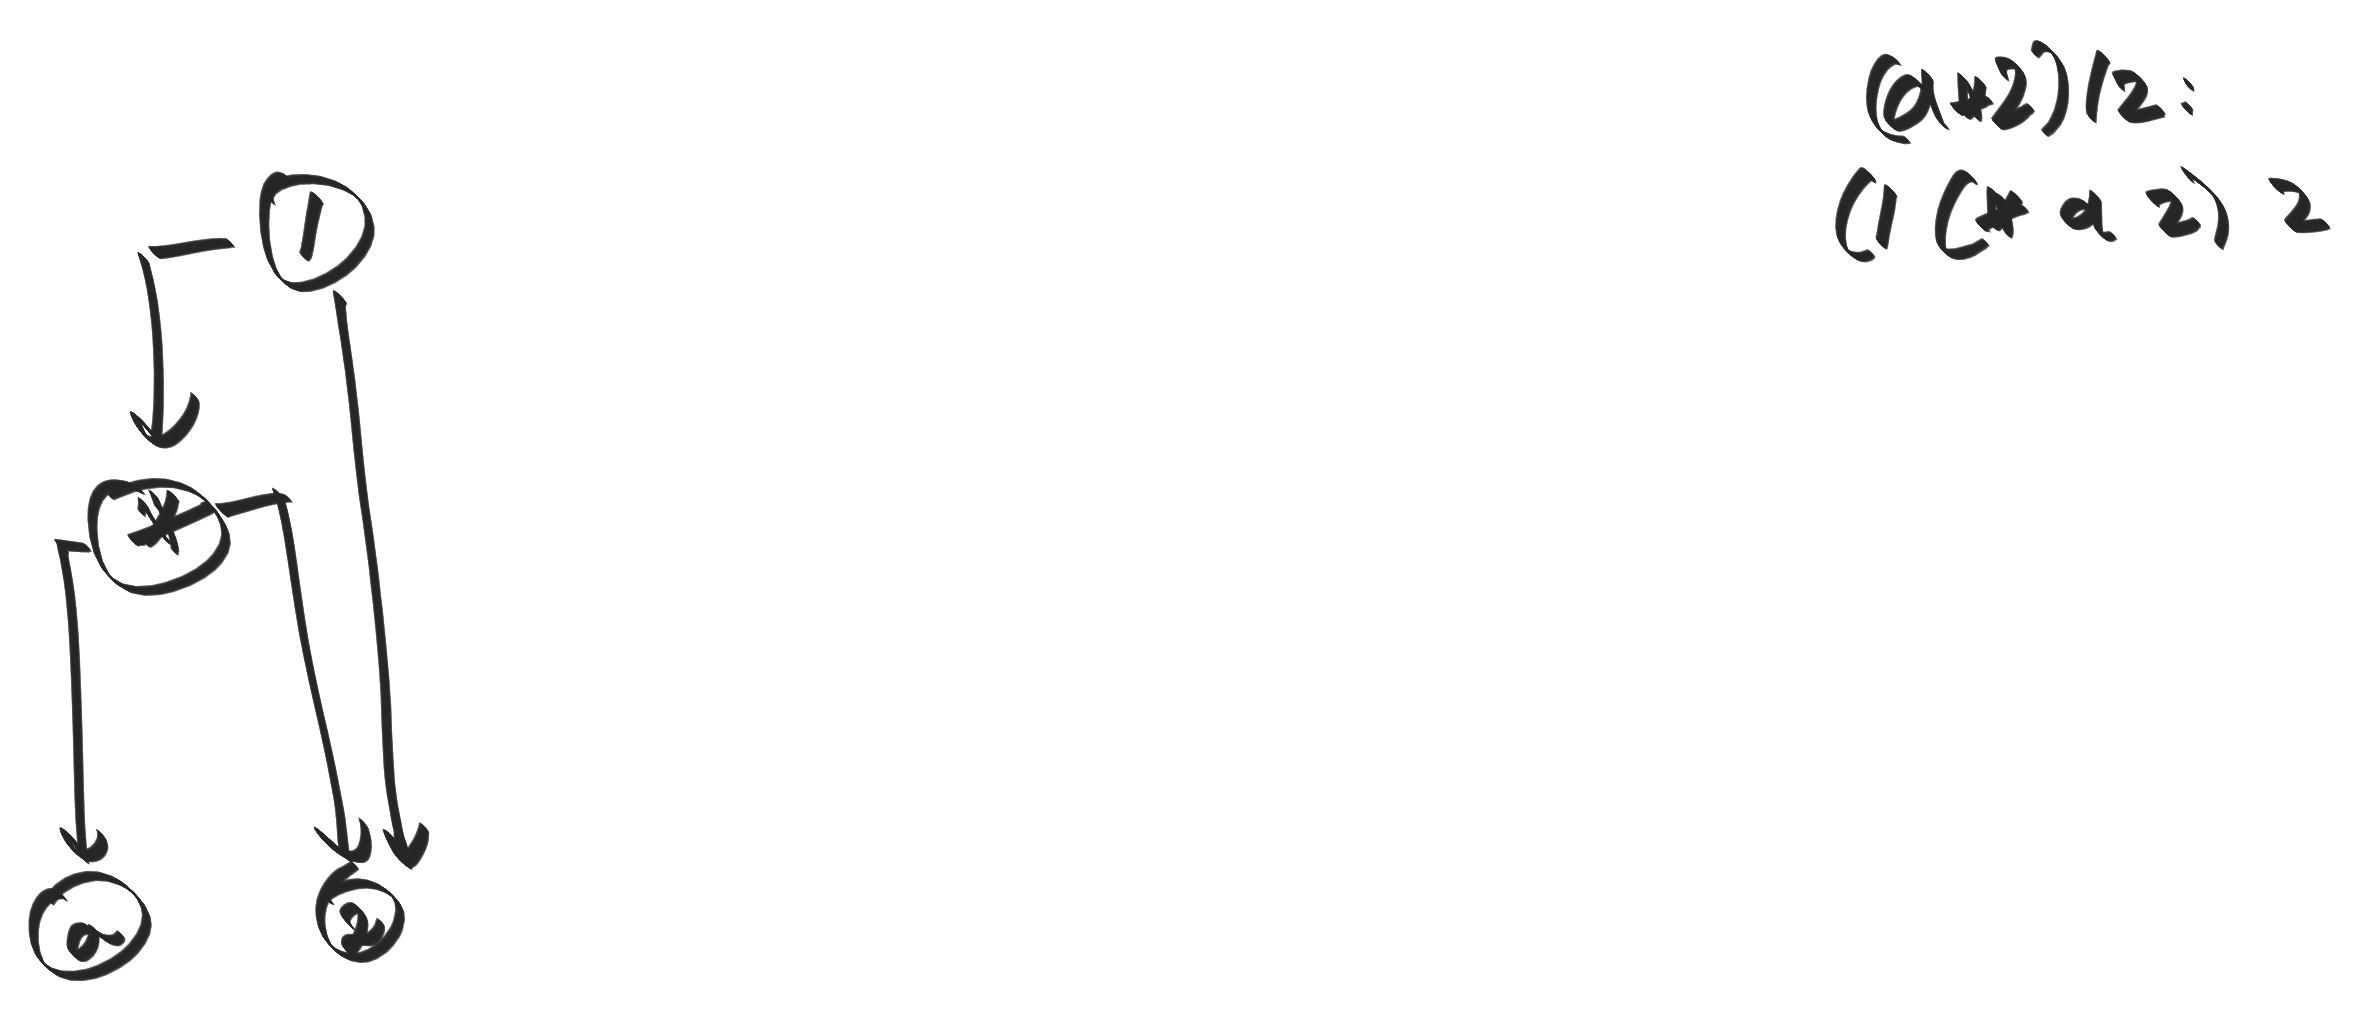
\includegraphics[width=\textwidth]{./eg-1-1.png}
\end{frame}

\begin{frame}[fragile]{\egg: Fast and extensible equality saturation (2)}
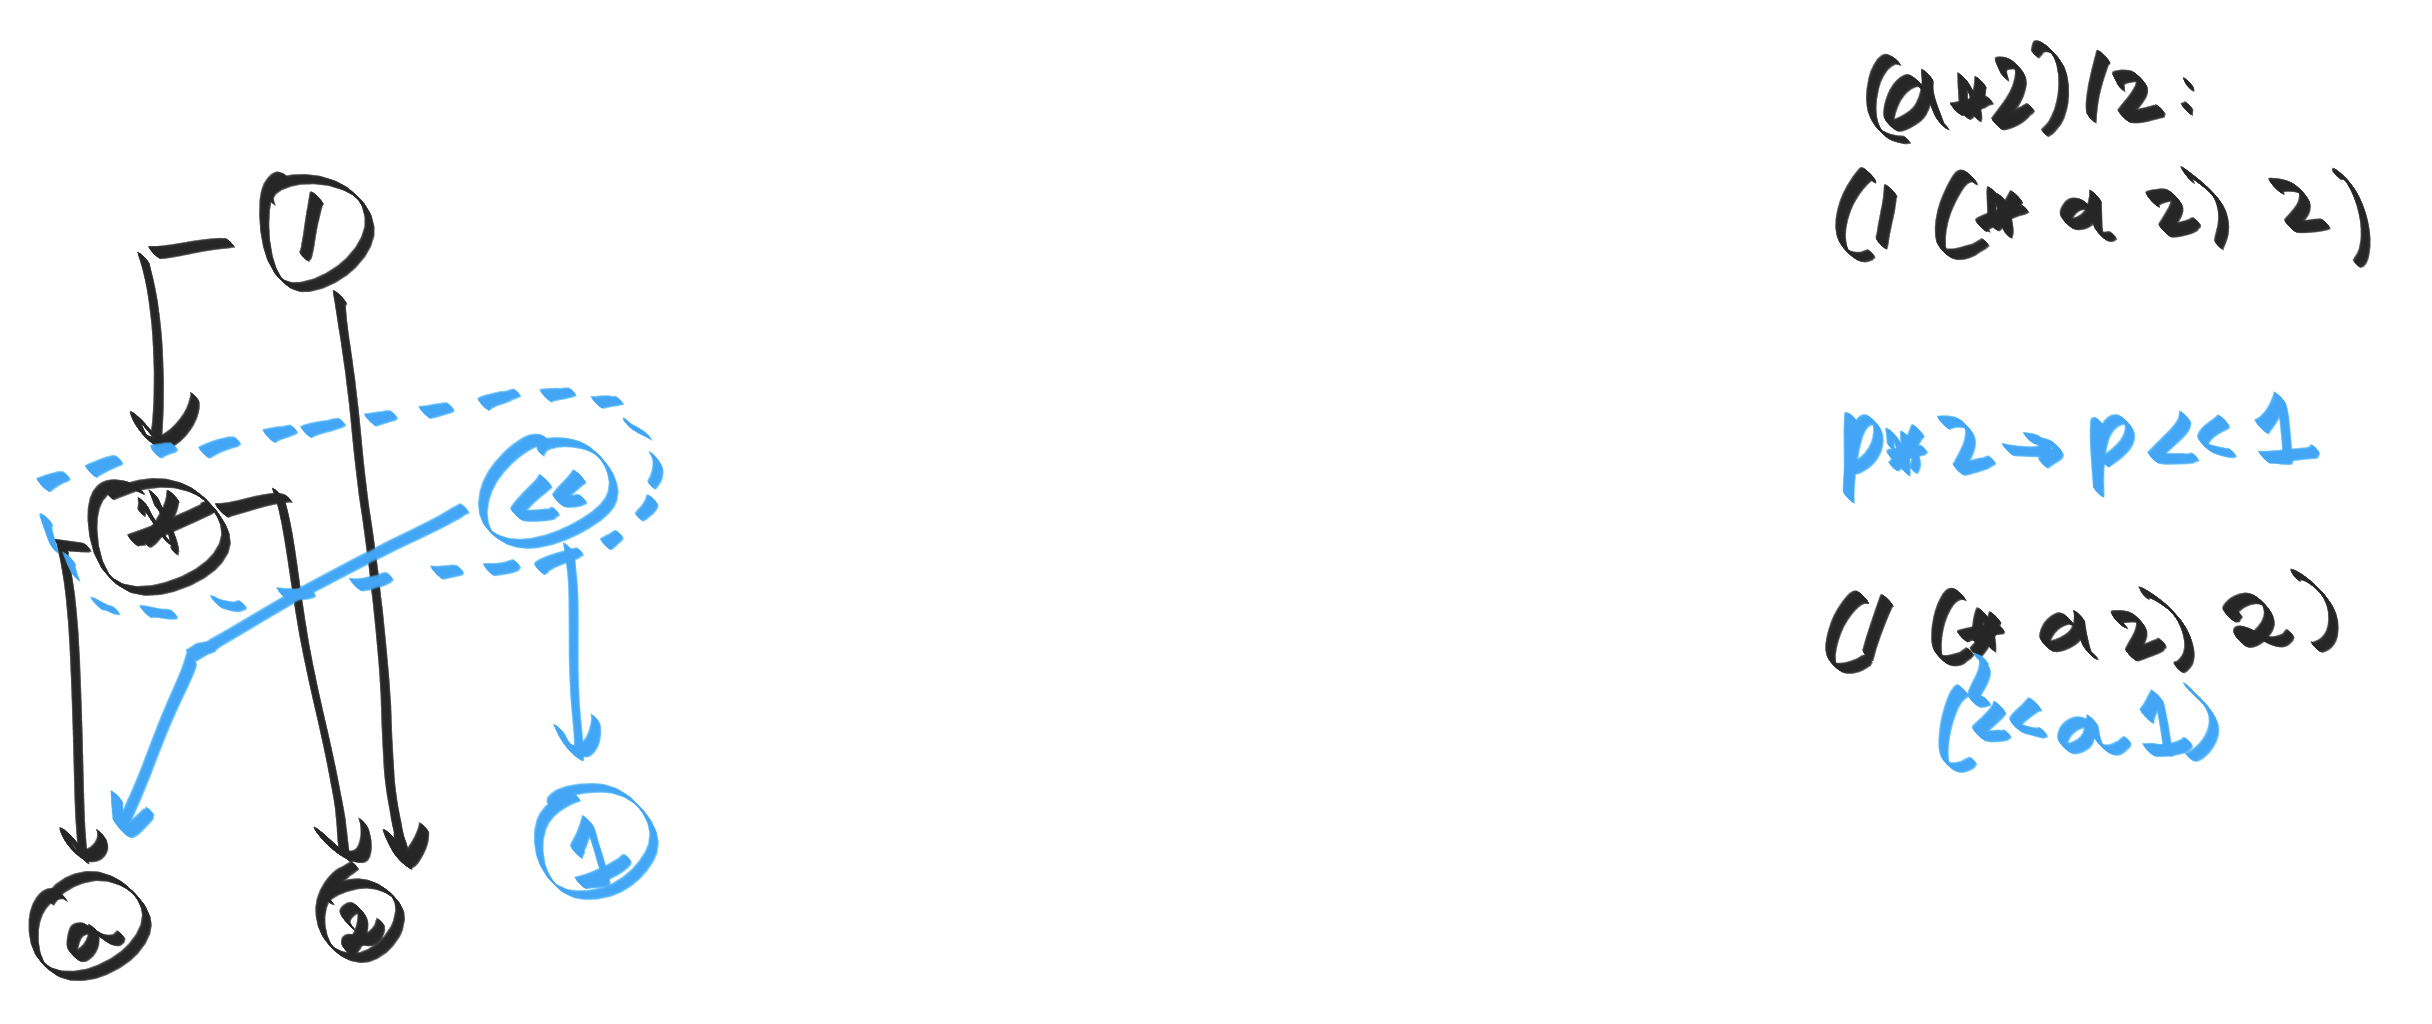
\includegraphics[width=\textwidth]{./eg-1-2.png}
\end{frame}


\begin{frame}[fragile]{\egg: Fast and extensible equality saturation (3)}
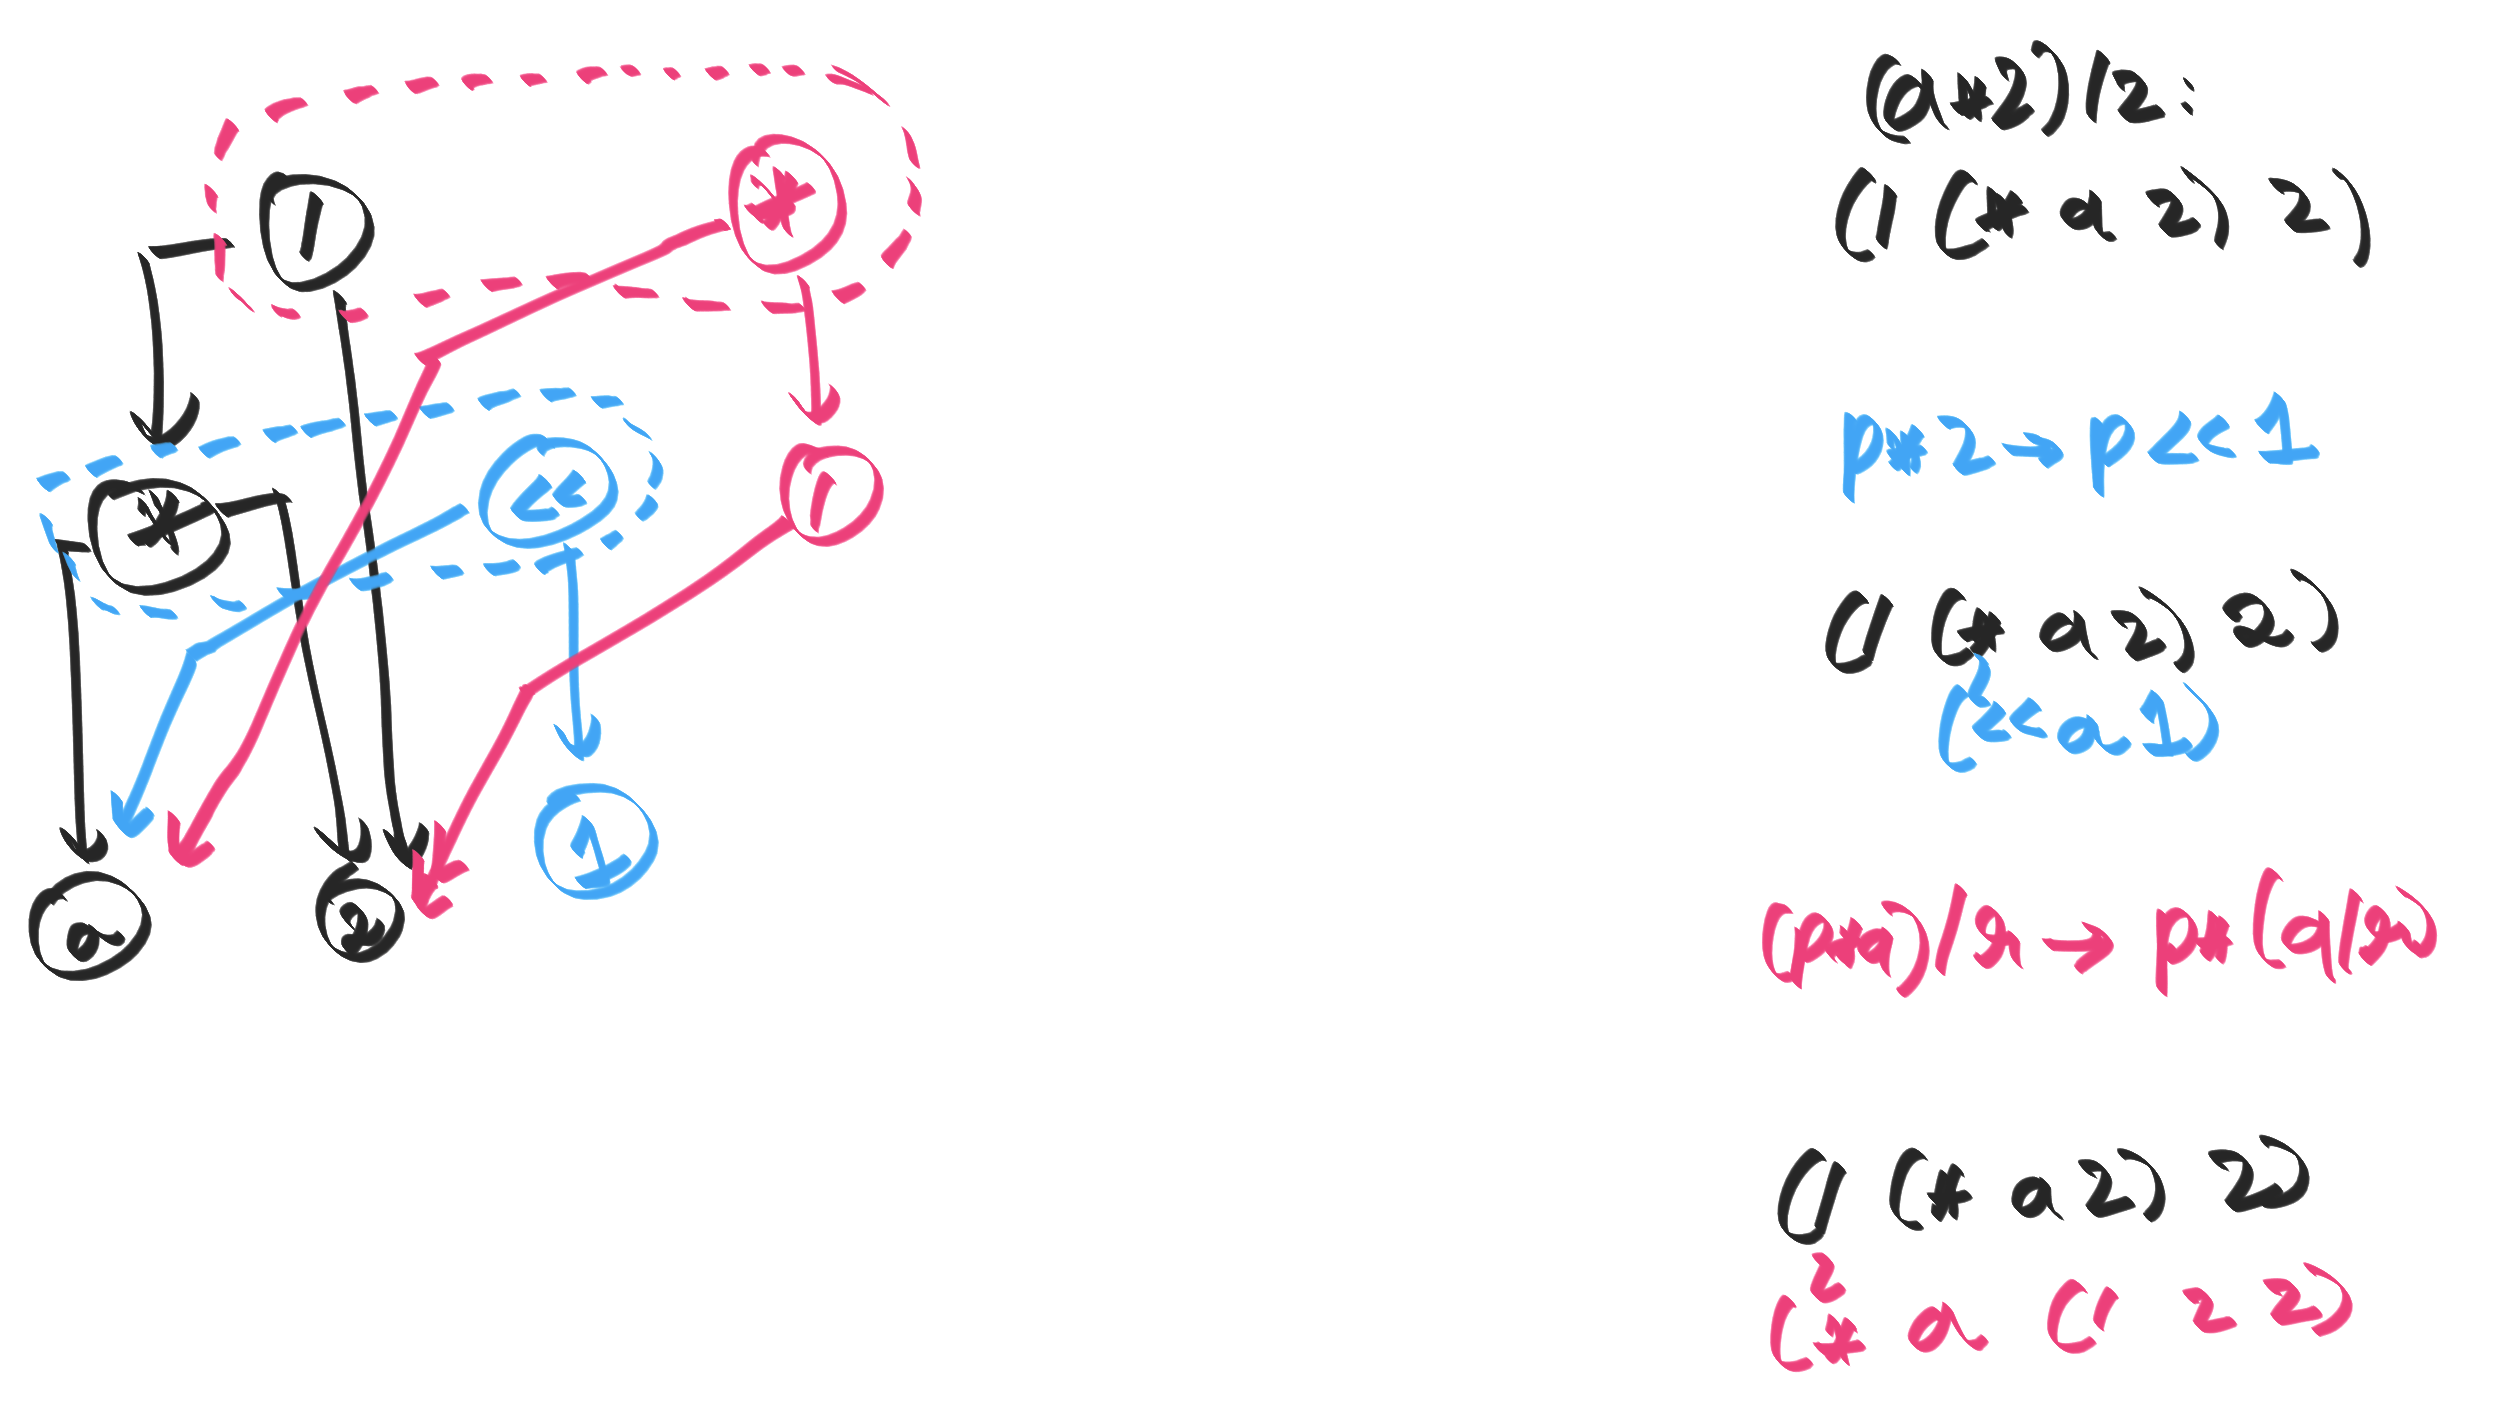
\includegraphics[width=\textwidth]{./eg-1-3.png}
\end{frame}

\begin{frame}[fragile]{\egg: Fast and extensible equality saturation (4)}
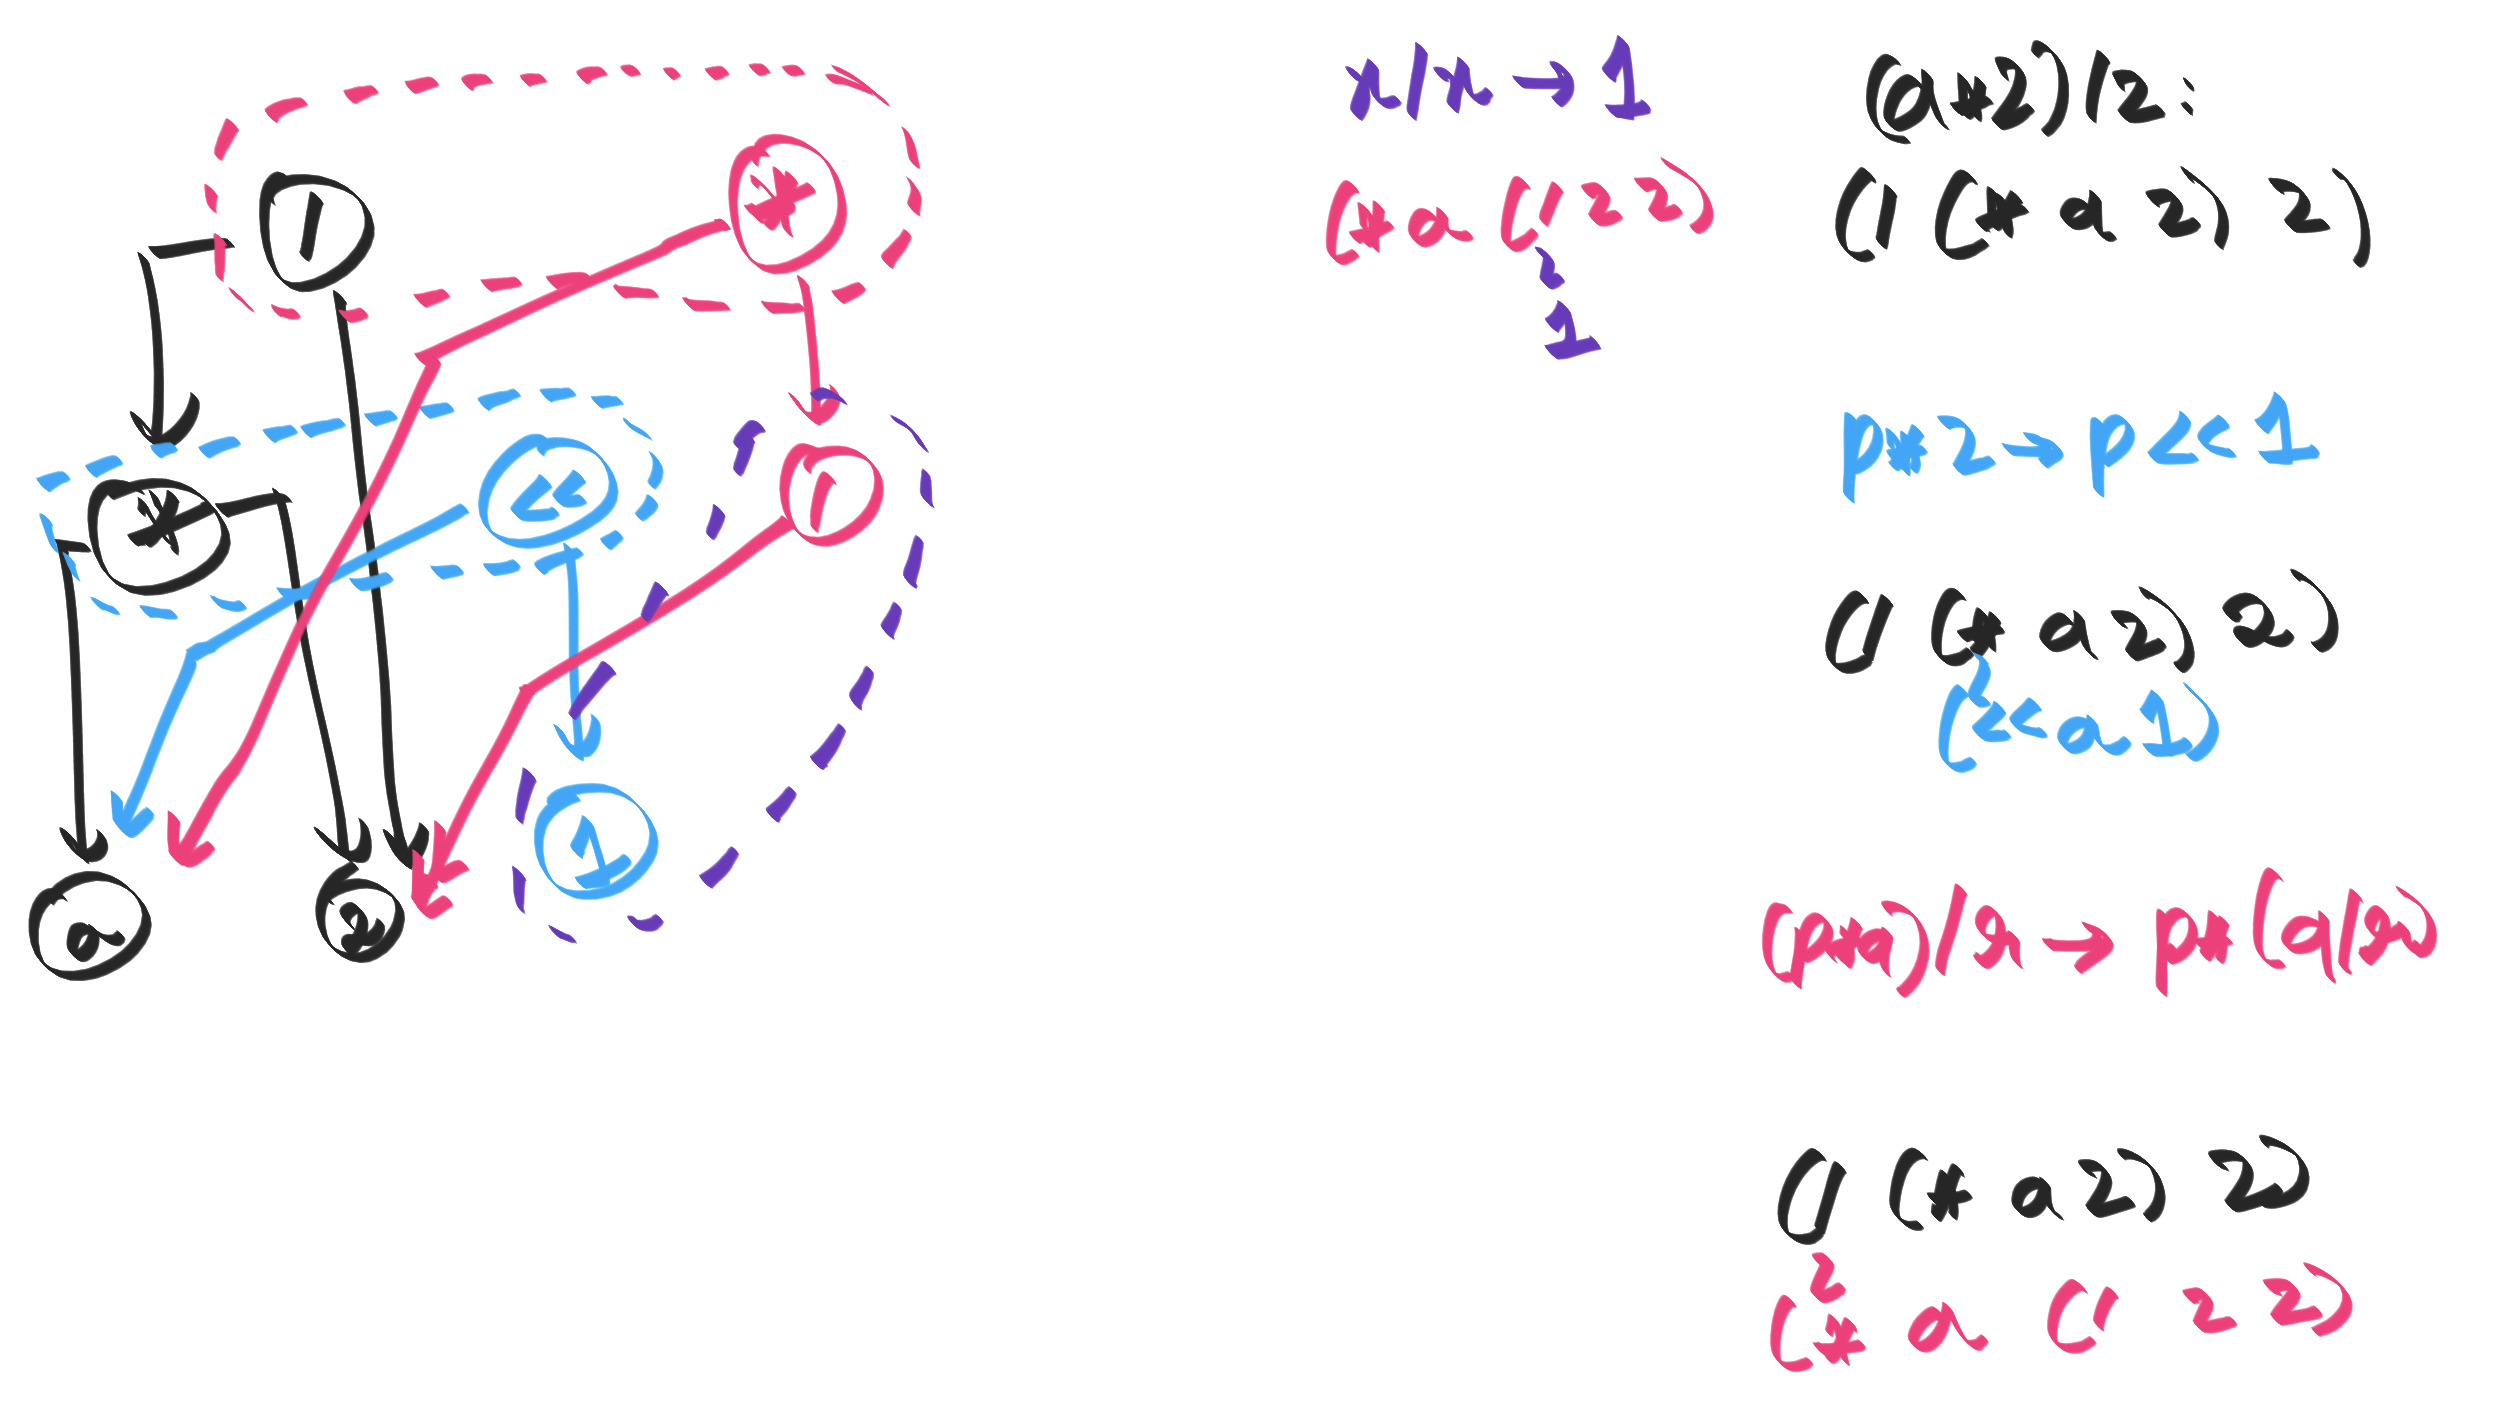
\includegraphics[width=\textwidth]{./eg-1-4.png}
\end{frame}


\begin{frame}[fragile]{\egg: Fast and extensible equality saturation (5)}
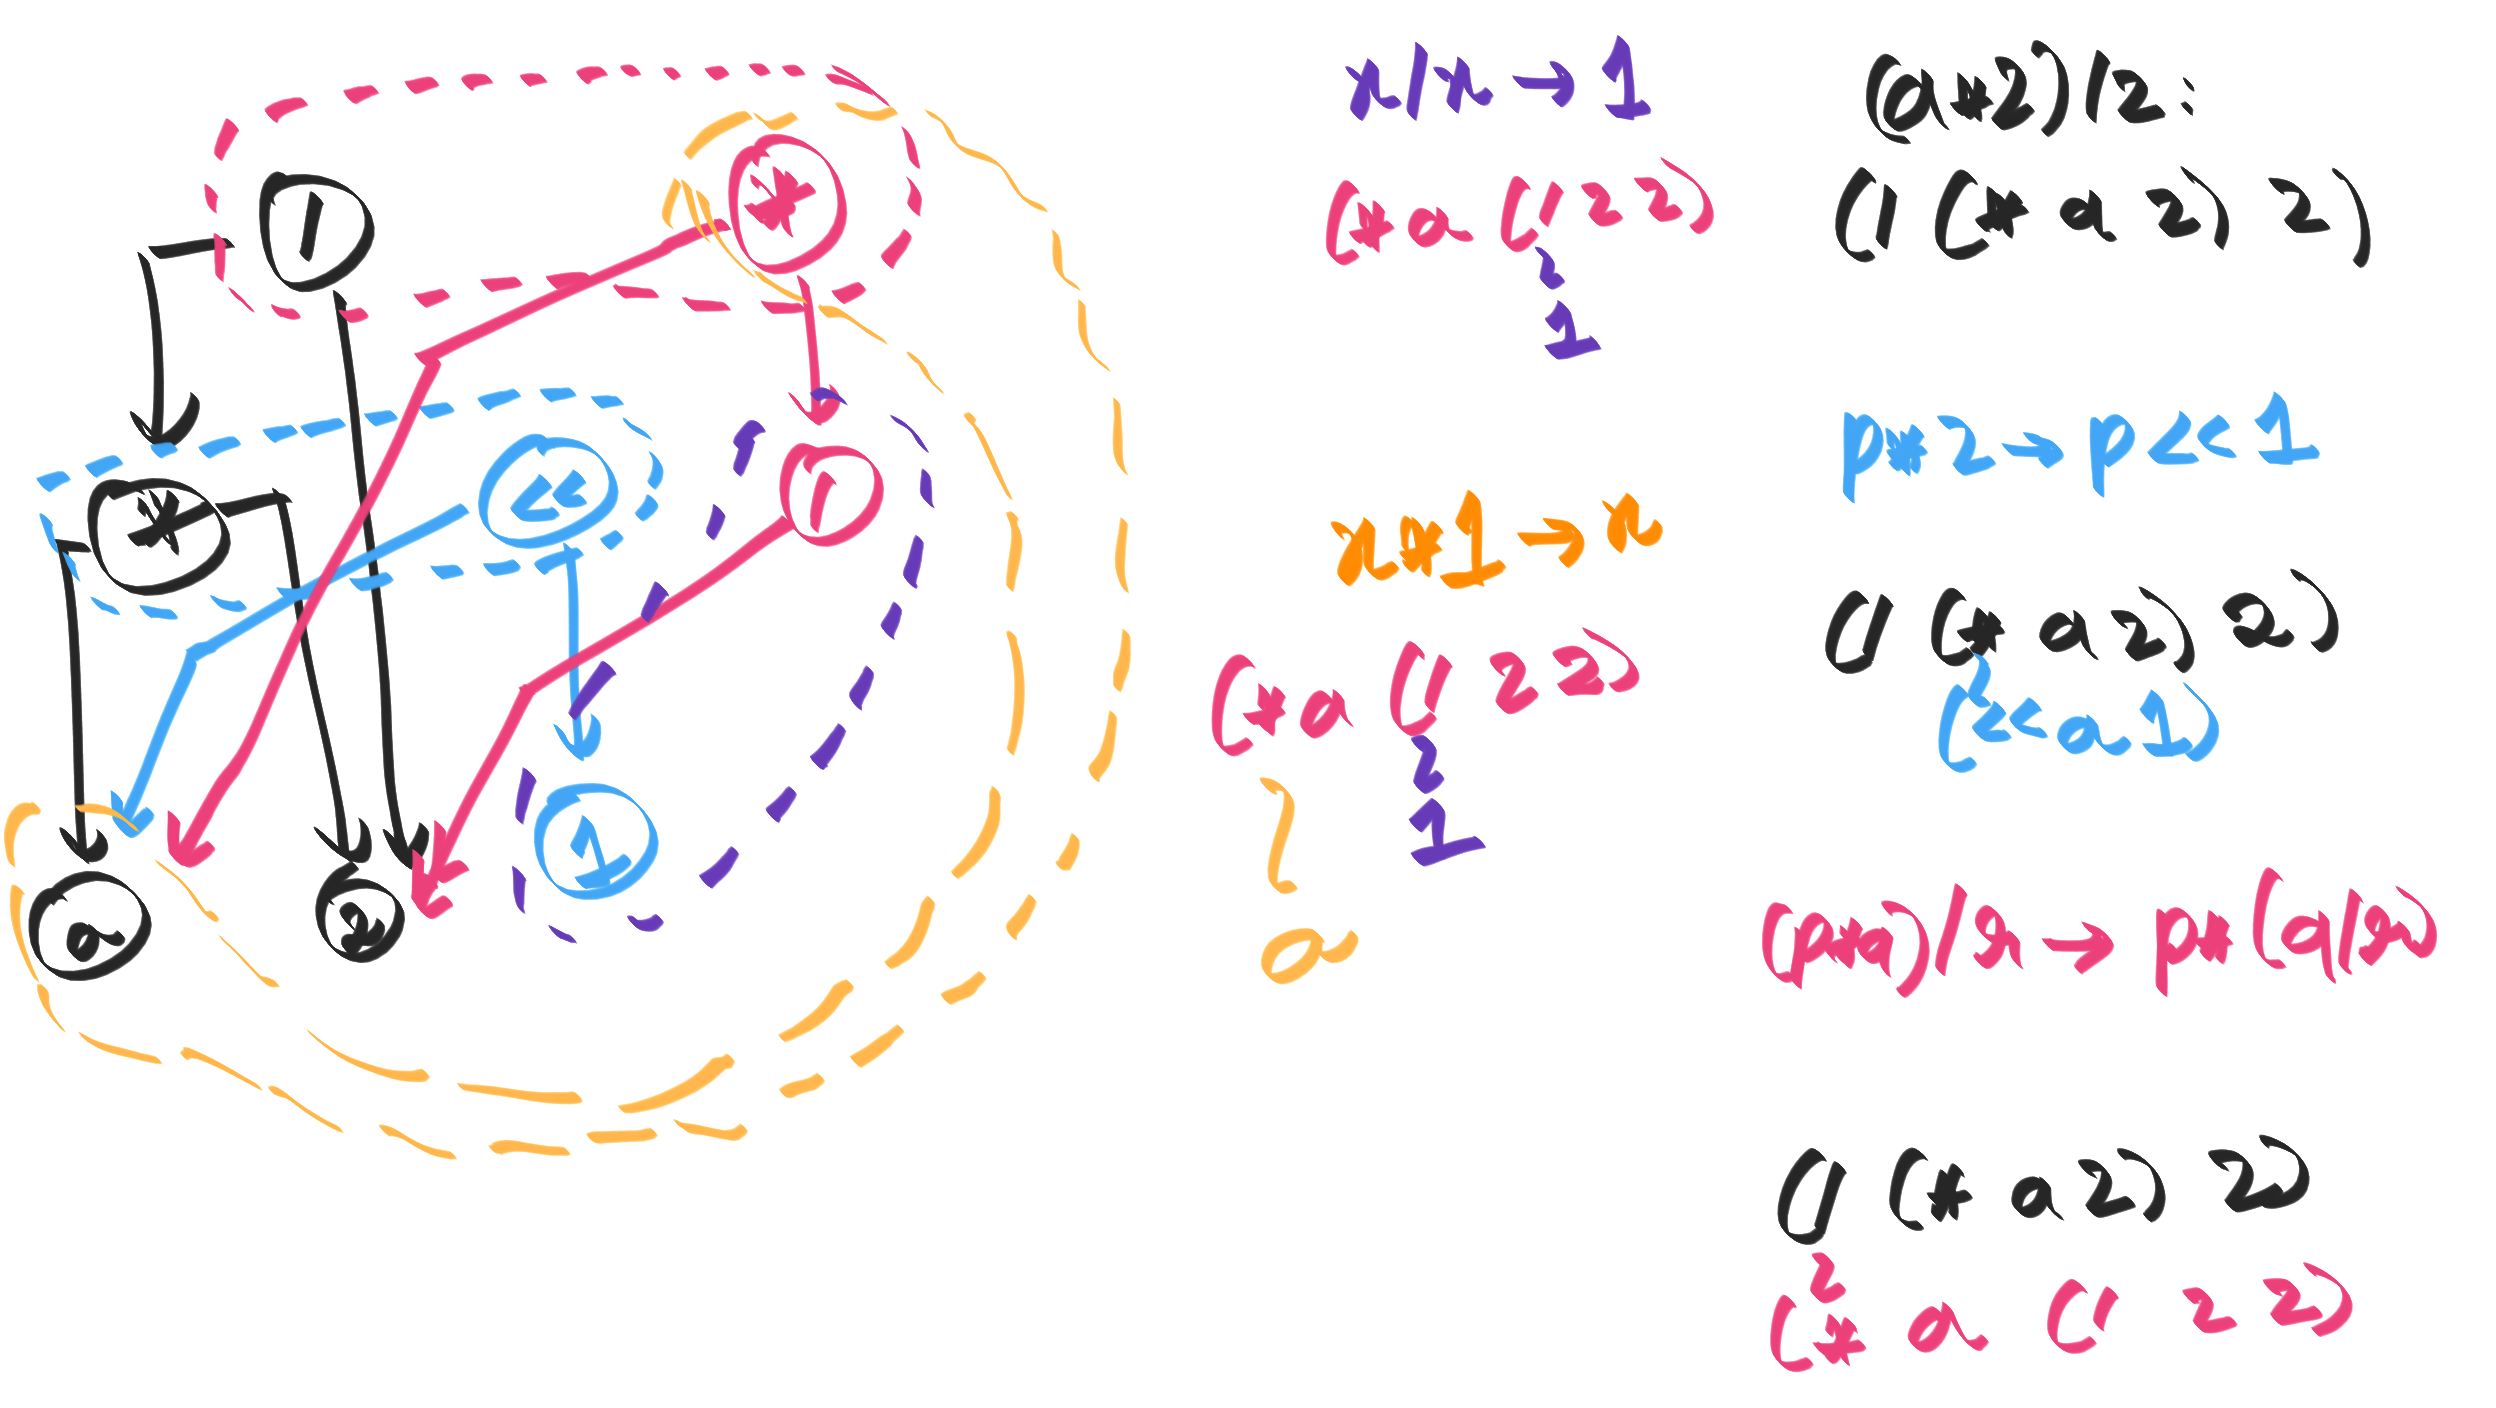
\includegraphics[width=\textwidth]{./eg-1-5.png}
\end{frame}


\begin{frame}[fragile]{\egg: Fast and extensible equality saturation (6)}
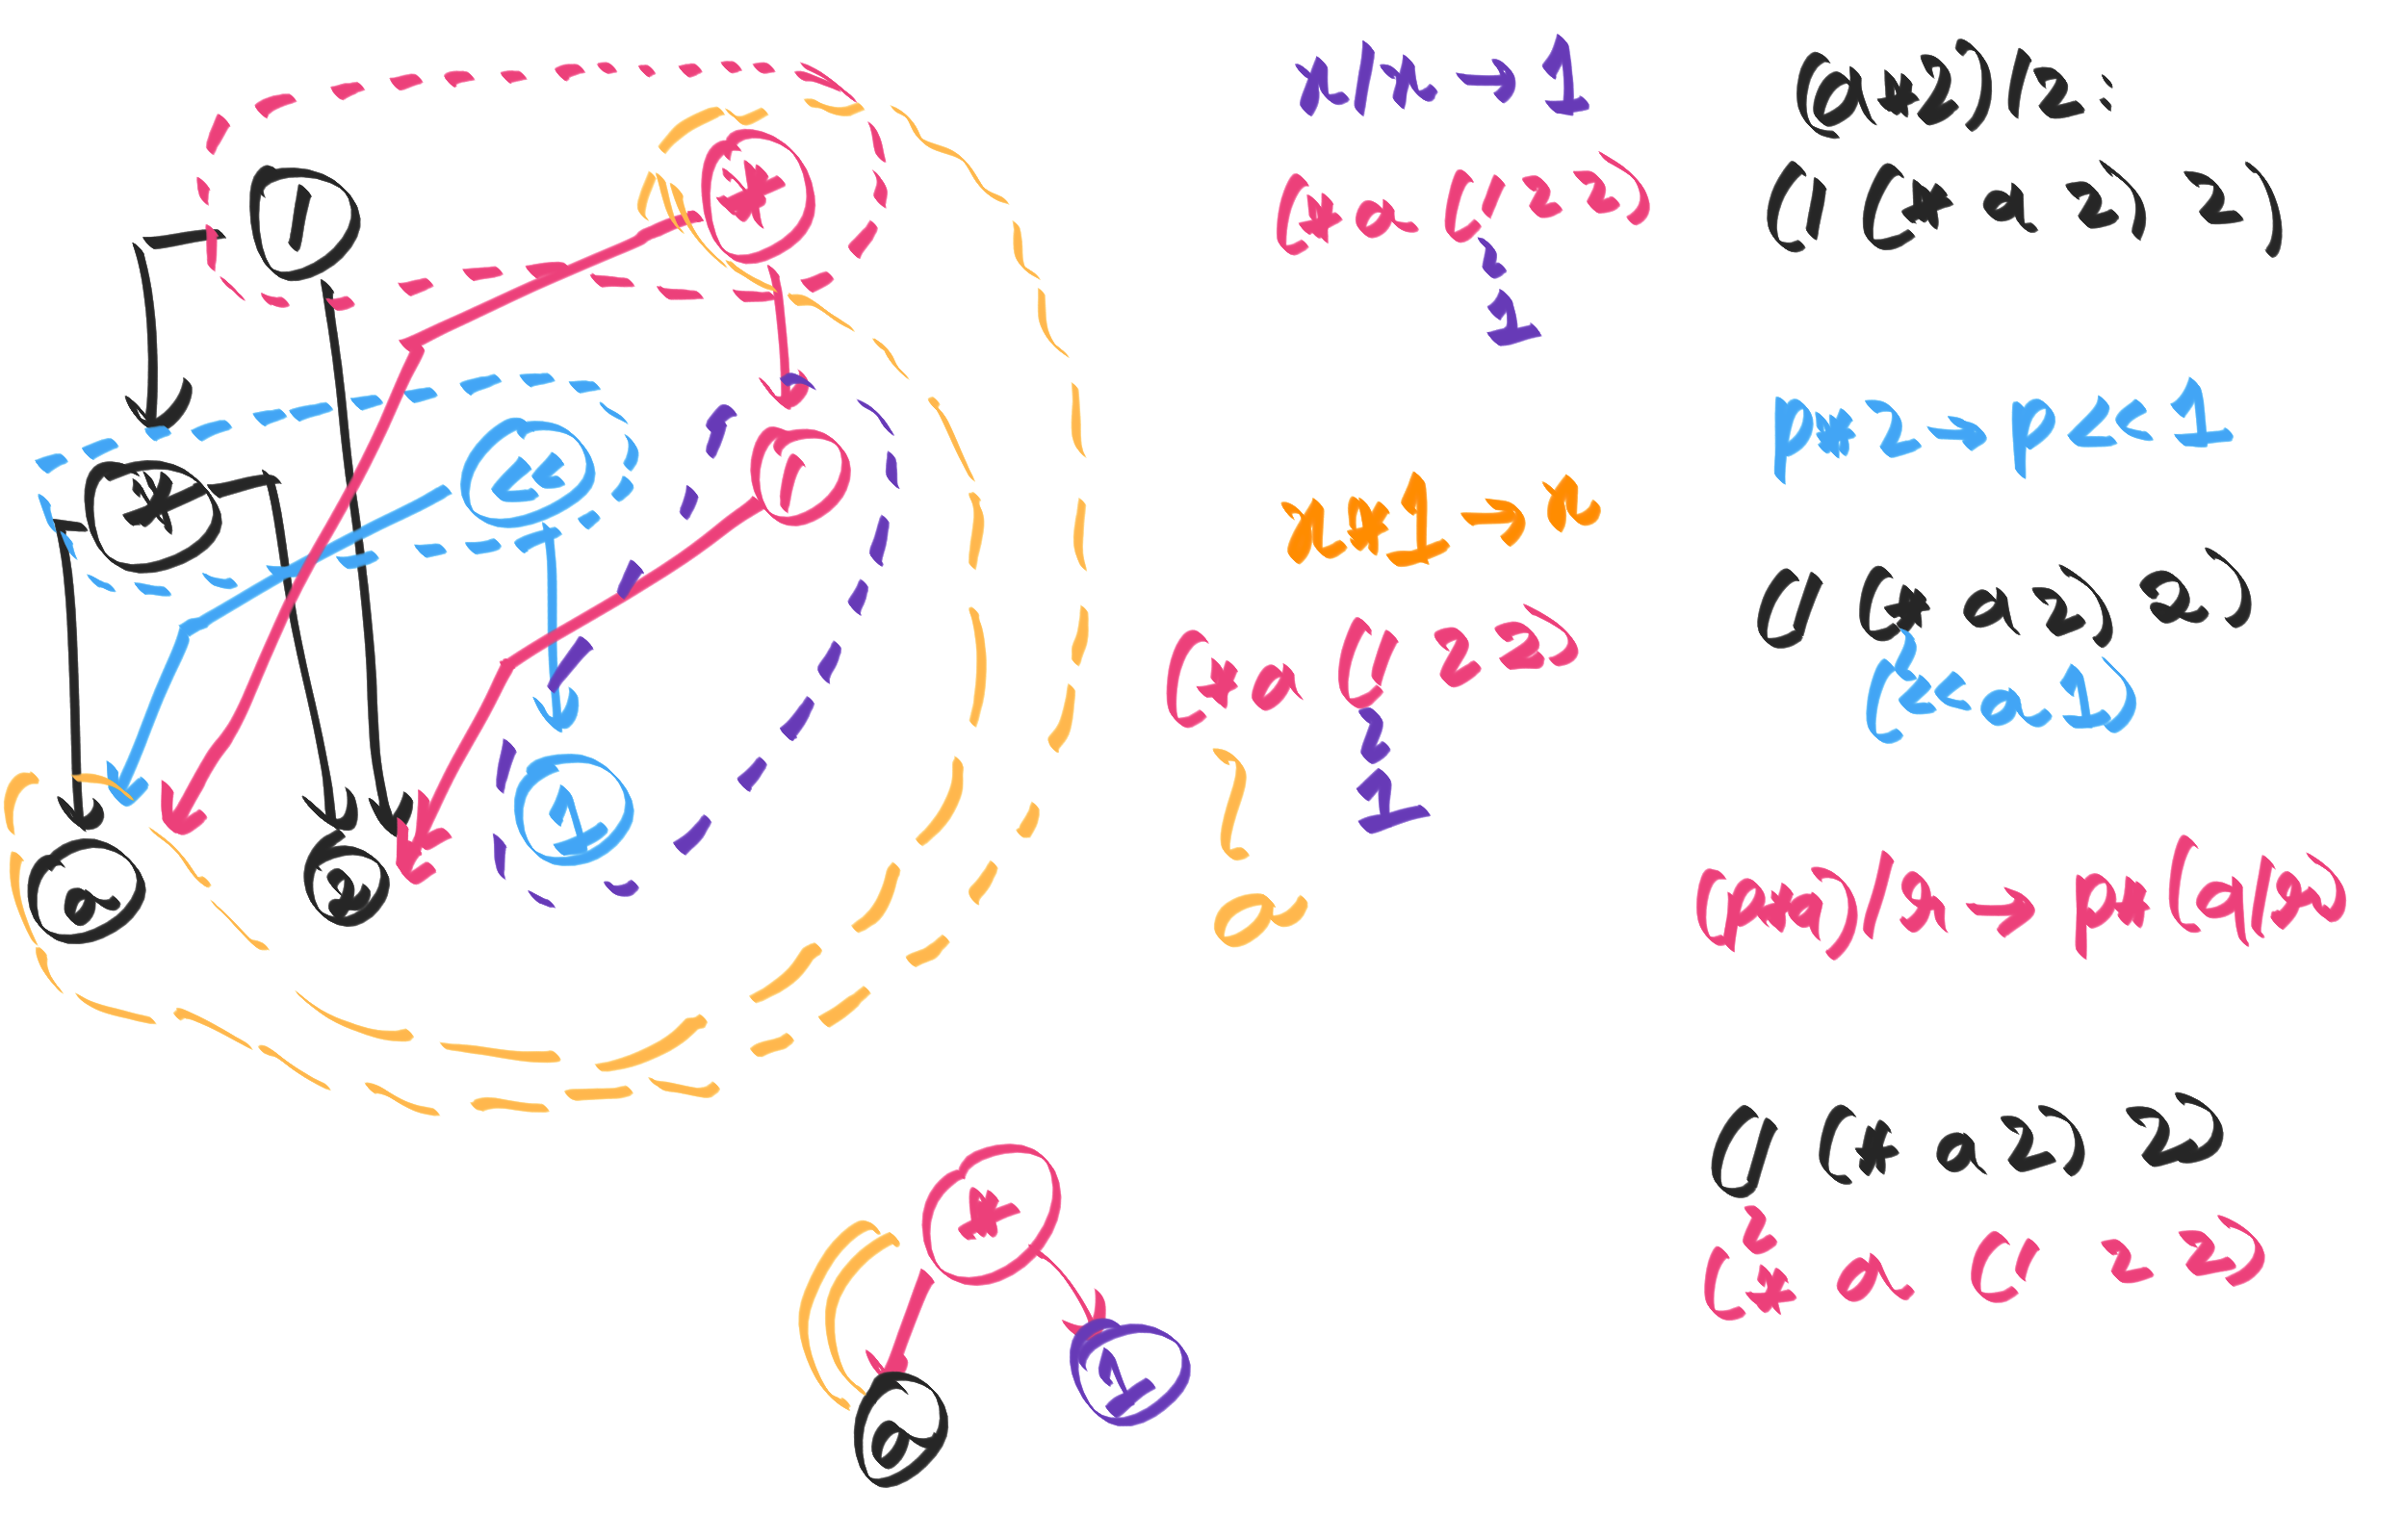
\includegraphics[width=\textwidth]{./eg-1-6.png}
\end{frame}

\begin{frame}[fragile]{\egg: Fast and extensible equality saturation (7)}
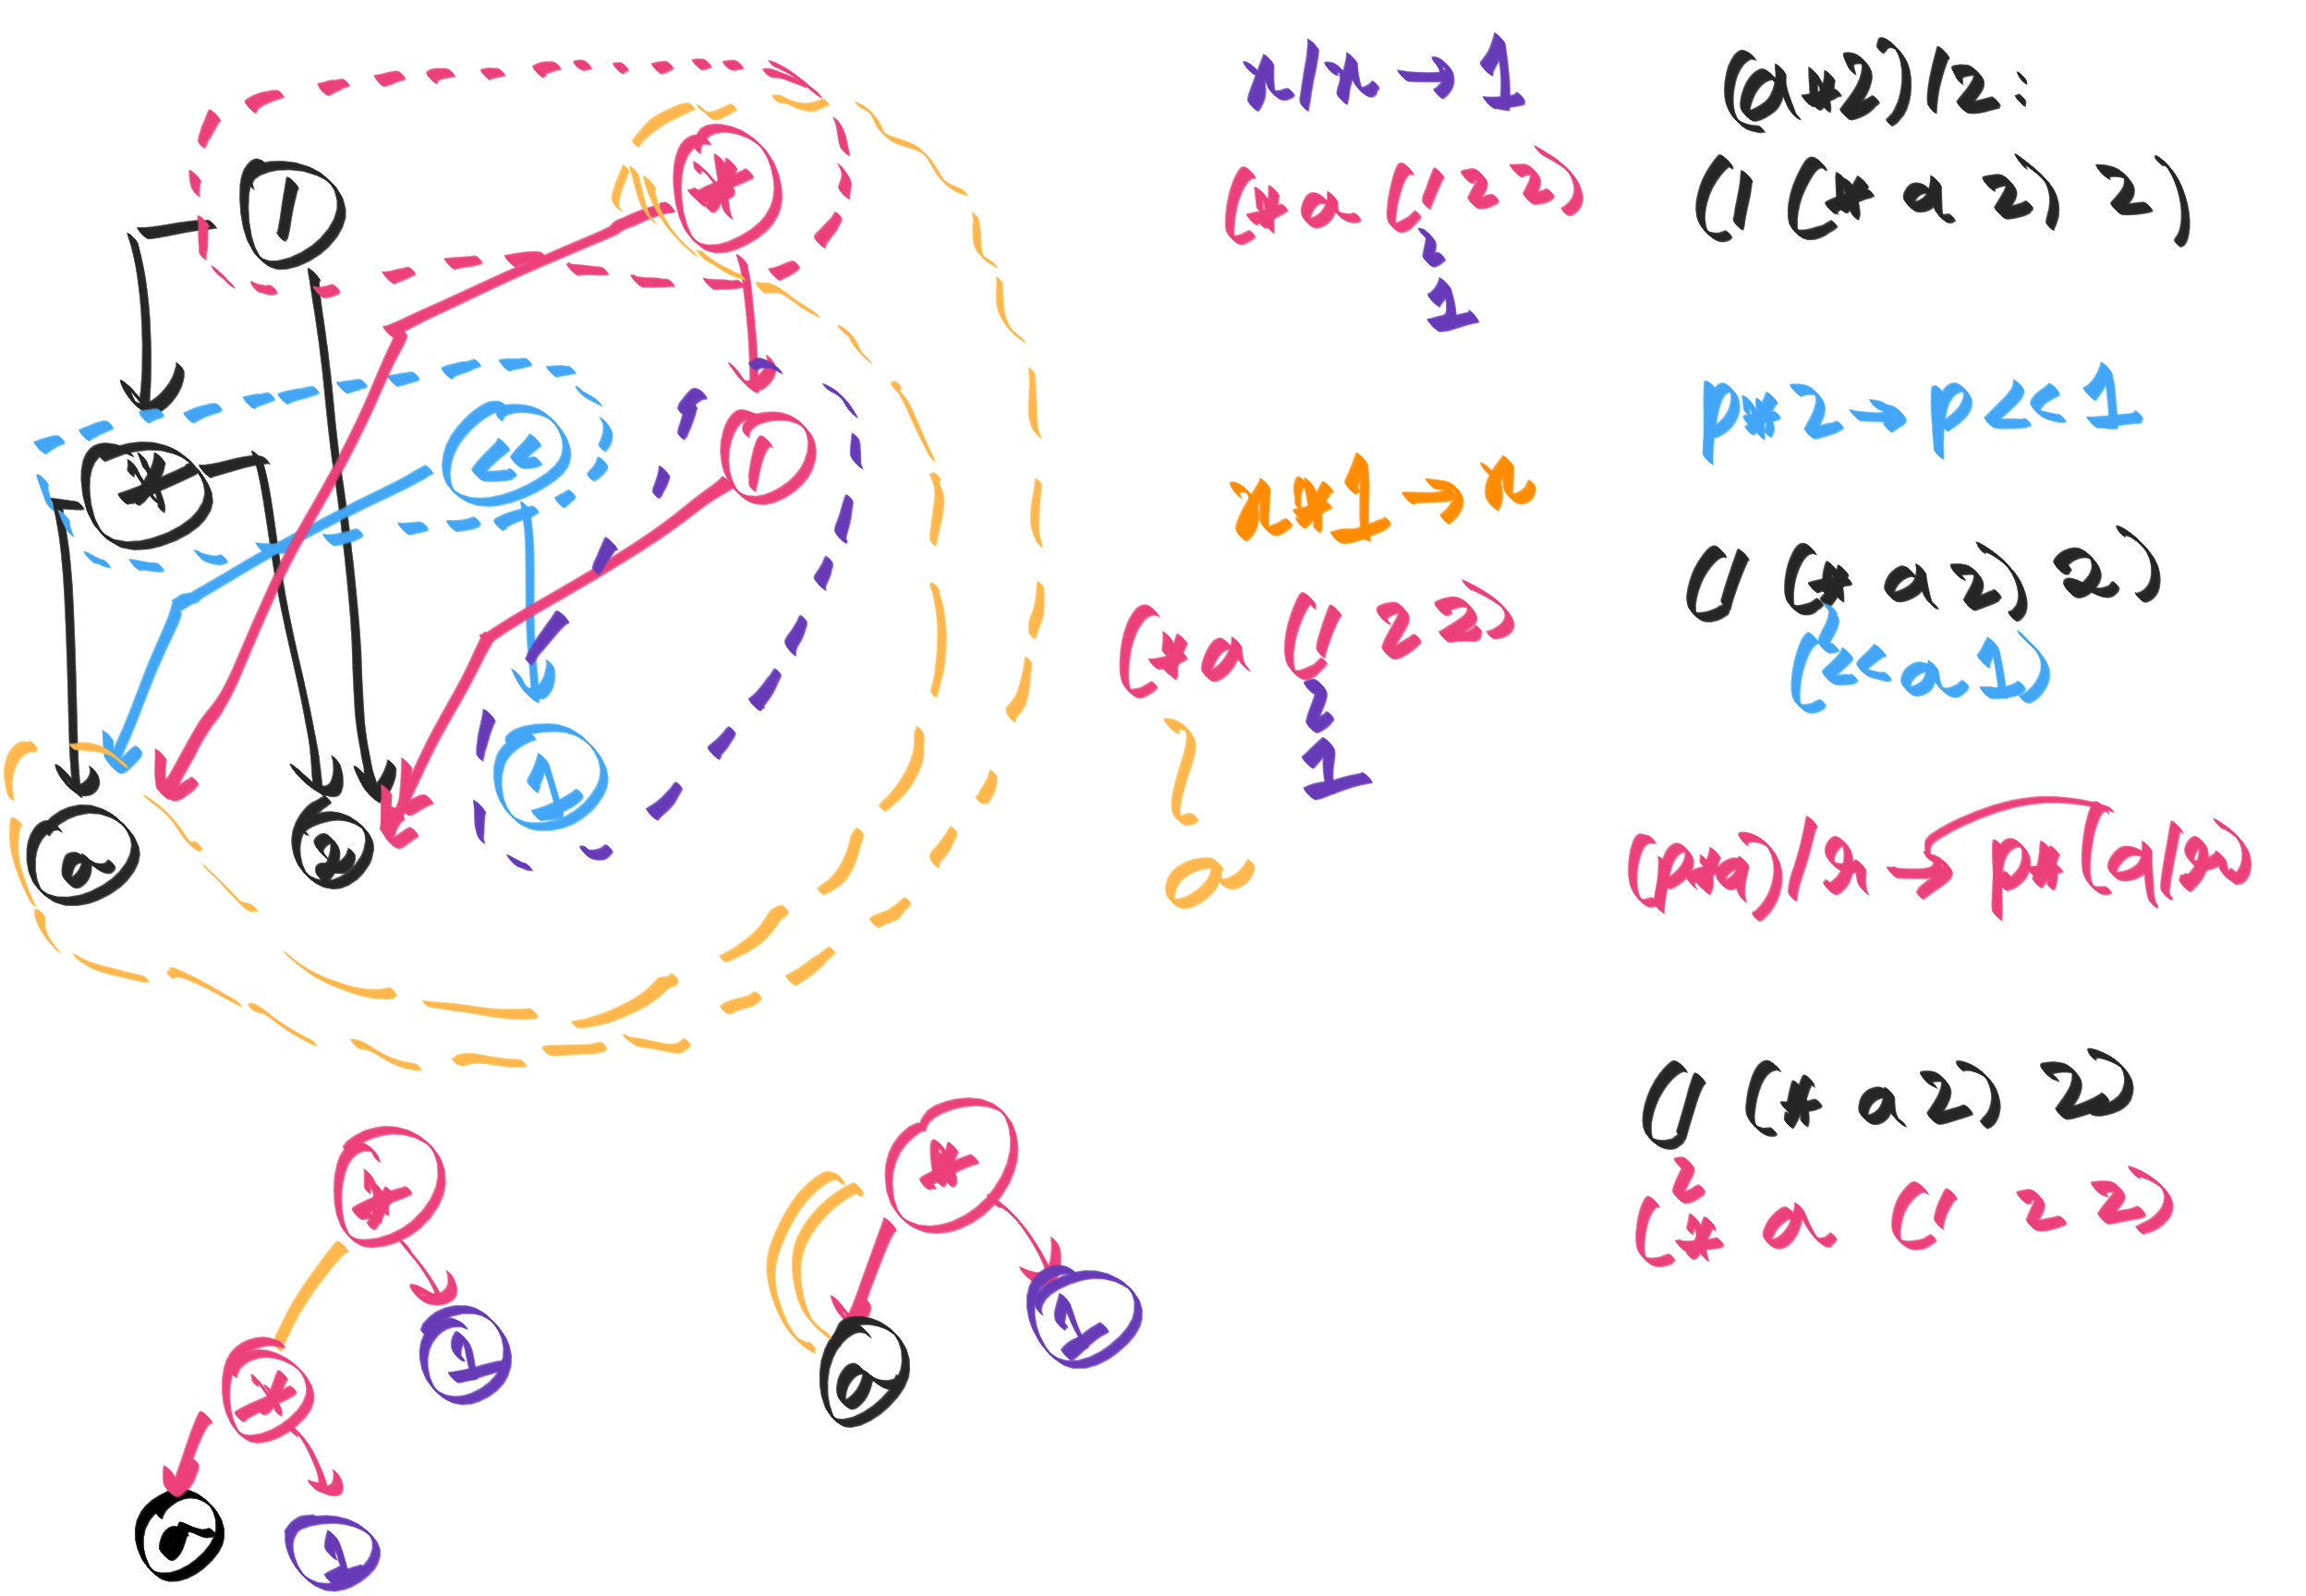
\includegraphics[width=\textwidth]{./eg-1-7.png}
\end{frame}


\begin{frame}[fragile]{\egg: Fast and extensible equality saturation (8)}
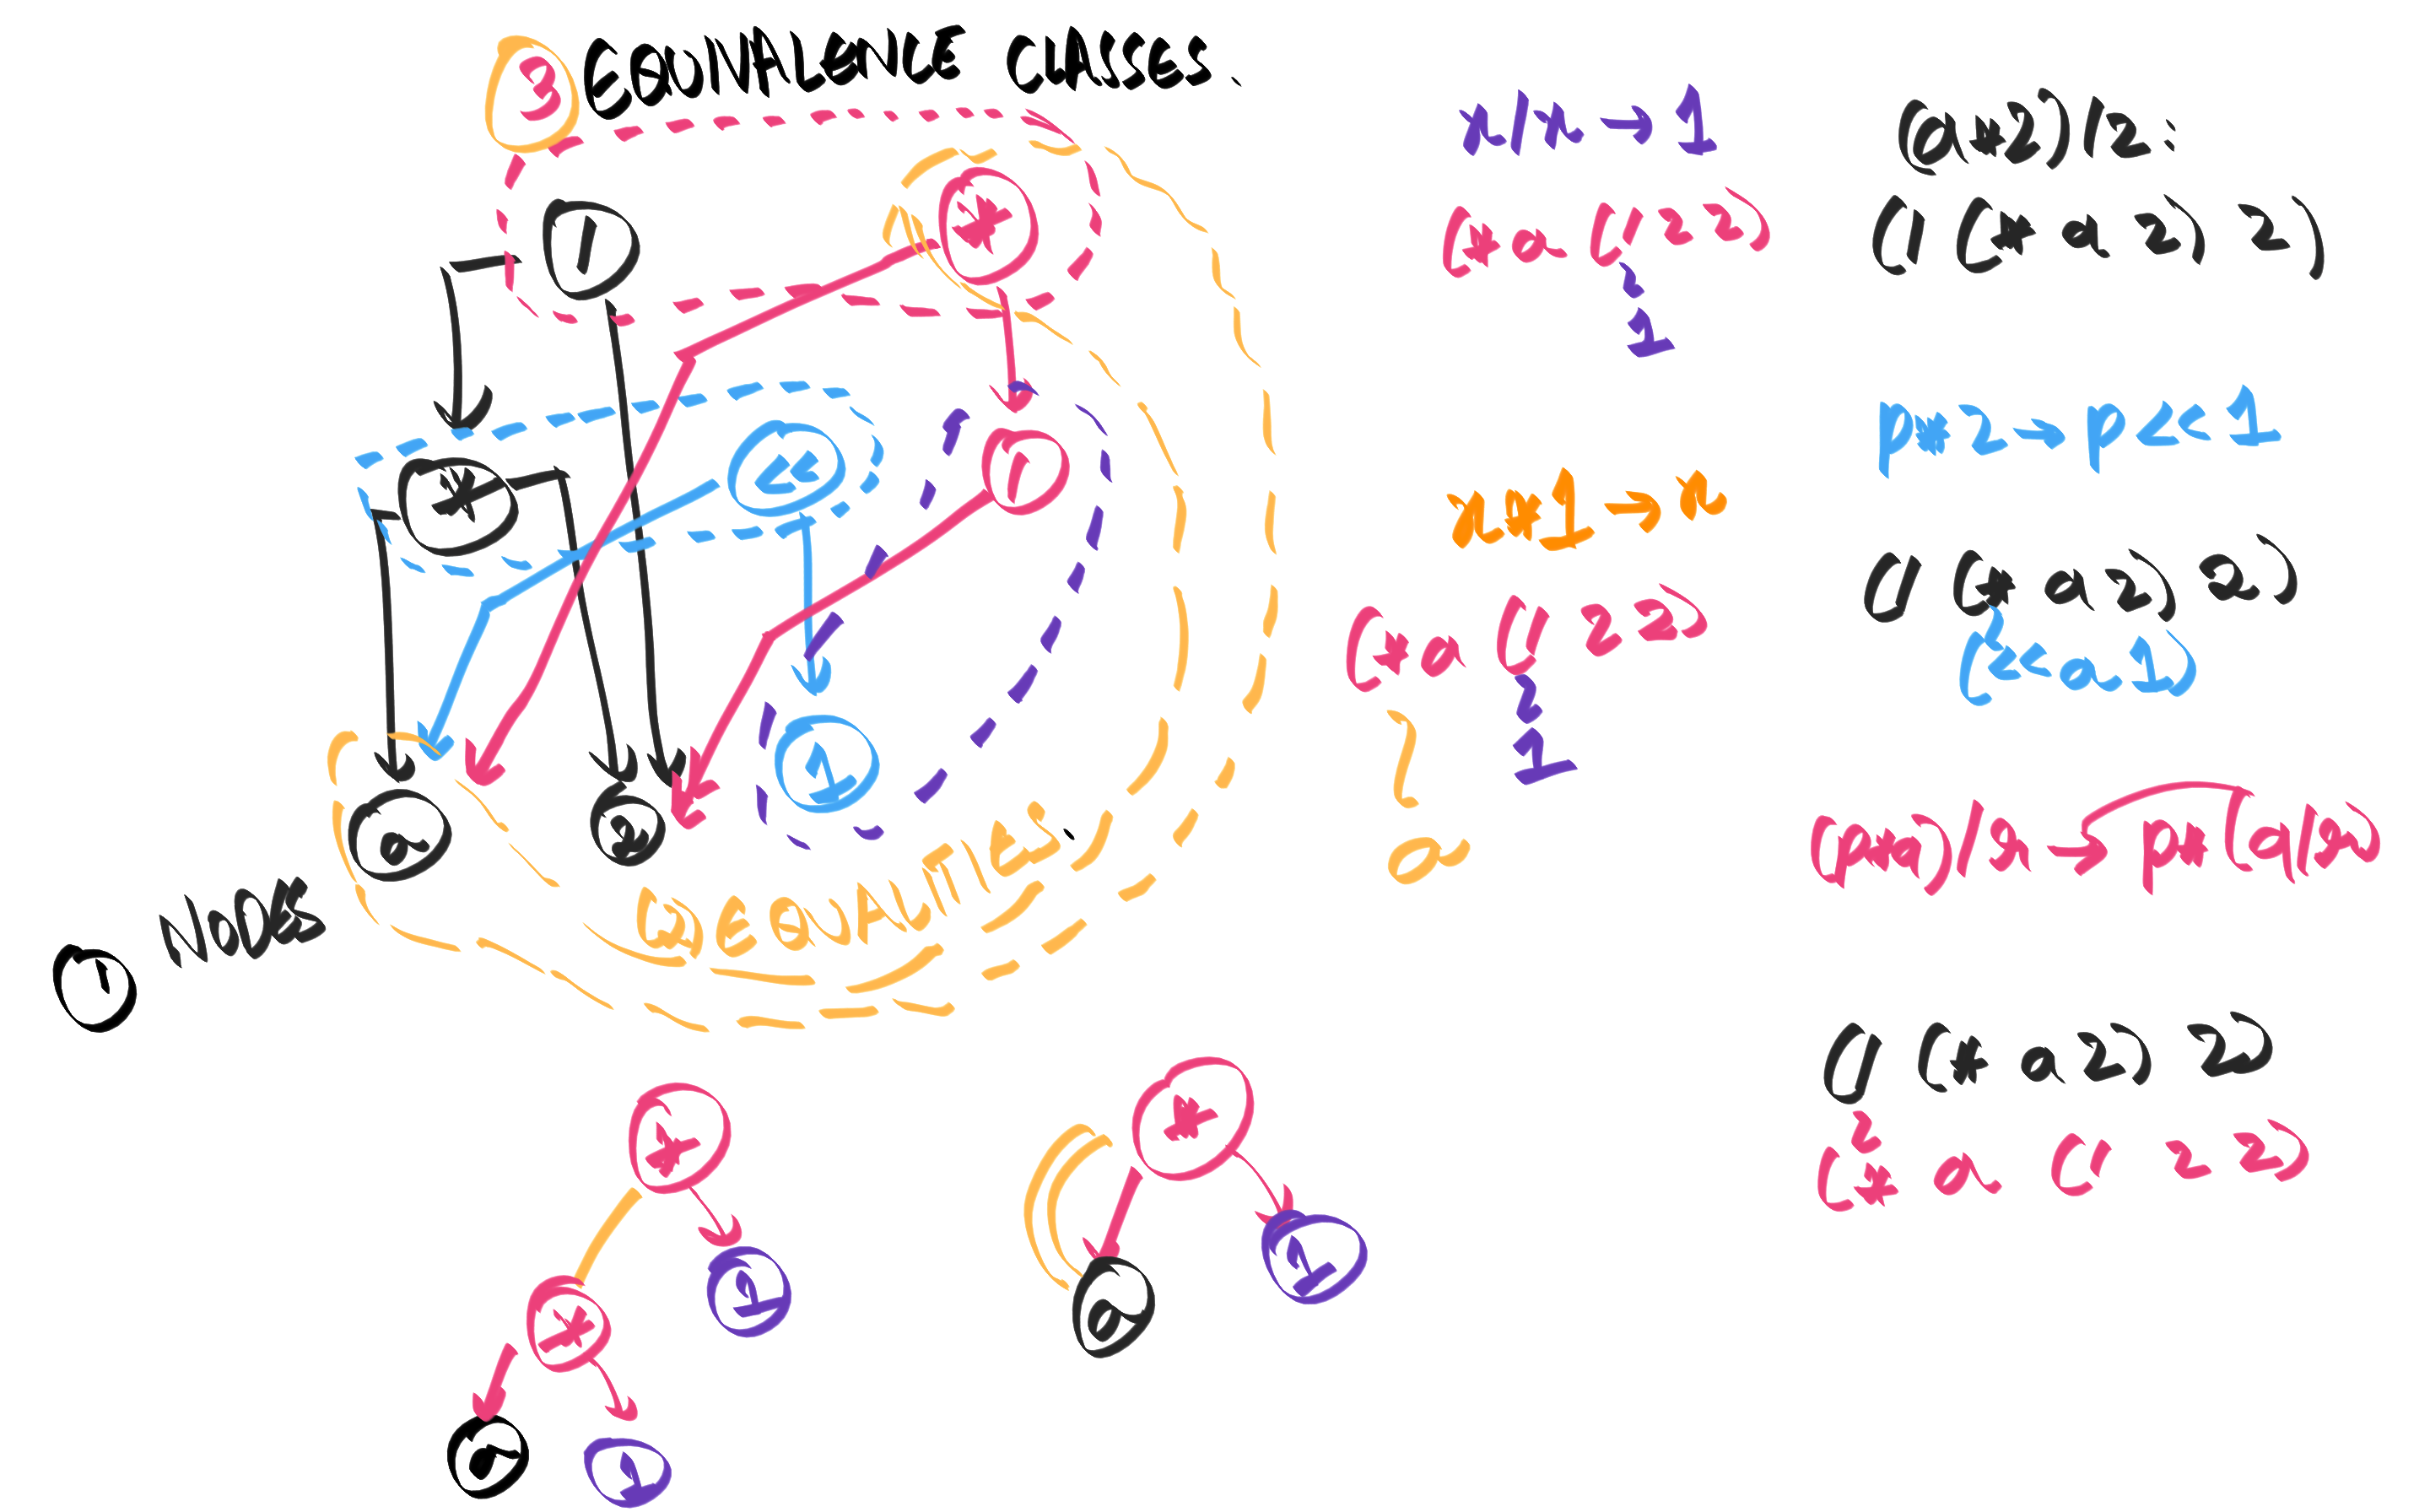
\includegraphics[width=\textwidth]{./eg-1-8.png}
\end{frame}


\begin{frame}{Evaluation: Herbie}
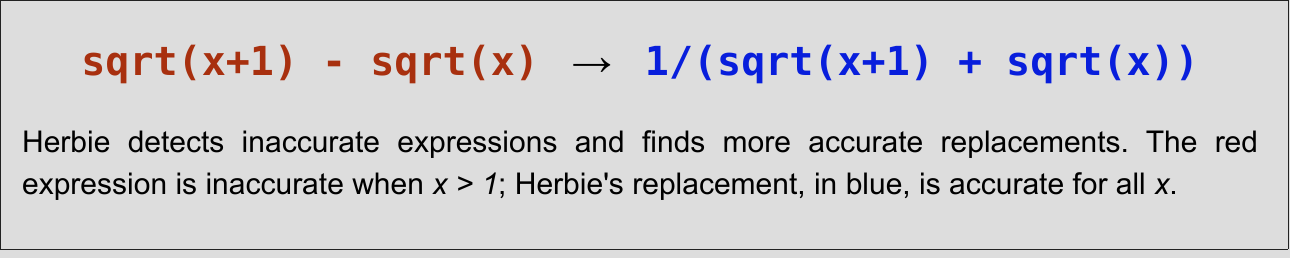
\includegraphics[width=\textwidth]{./herbie-sales-pitch.png}
\pause

$$
\sqrt{x+1}-\sqrt{x} =
\frac{(\sqrt{x+1}-\sqrt{x})(\sqrt{x+1}+\sqrt{x})}{\sqrt{x+1}+\sqrt{x}}
= \frac{(x+1)-x}{\sqrt{x+1}+\sqrt{x}} = \frac{1}{(\sqrt{x+1}+\sqrt{x})}
$$
\pause
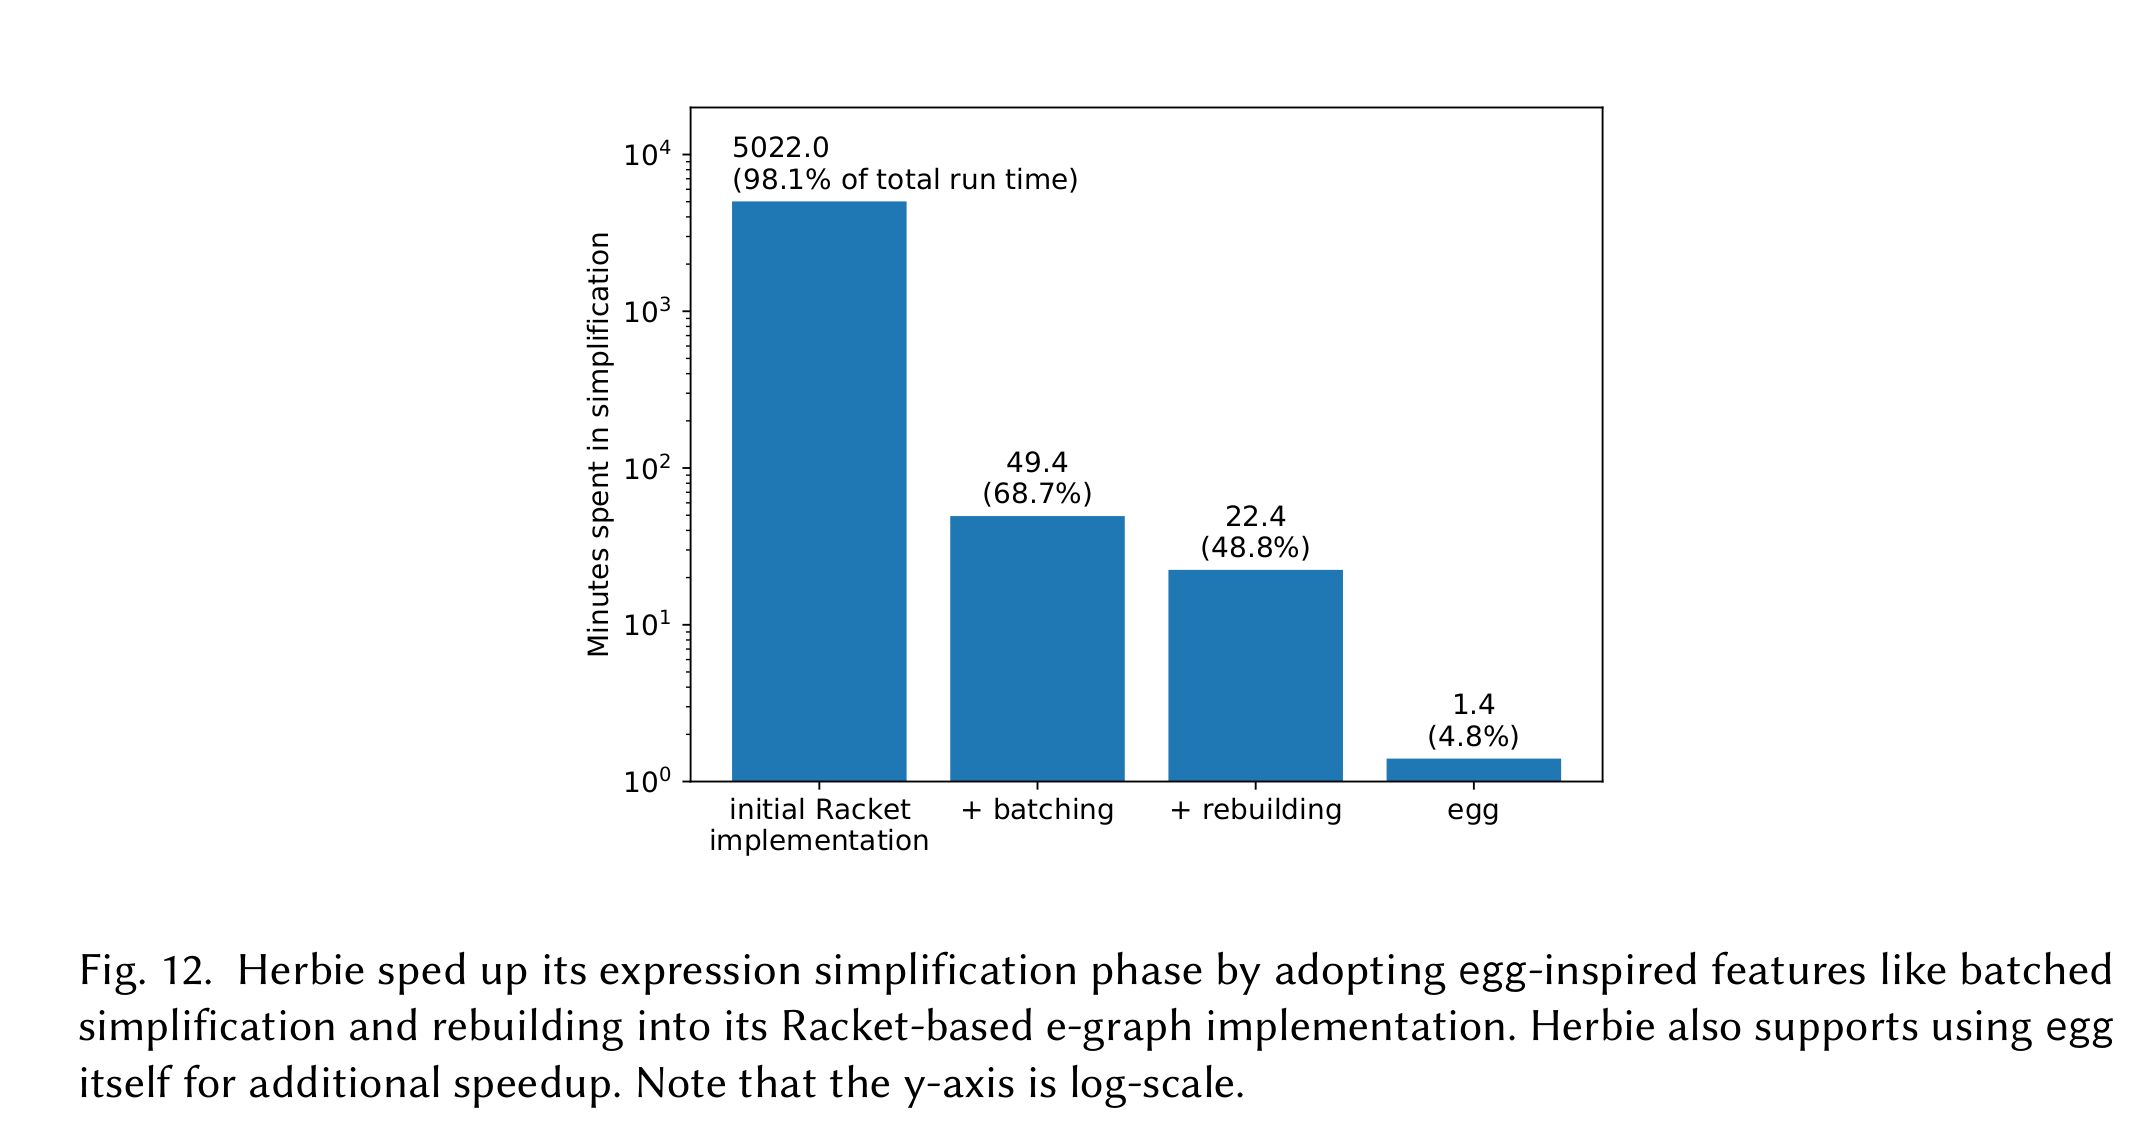
\includegraphics[width=0.8\textwidth]{./herbie-speedup.png}

\end{frame}

\begin{frame}[fragile]{Herbie: Using \egg --- rules}
\url{https://github.com/uwplse/herbie/blob/master/egg-herbie/src/rules.rs}

\begin{minted}{racket}
;; projections
("real-part","(re real (complex real ?x ?y))","?x")
;; why duplication of real and complex rules?
("associate-+r+.c", "(+ c ?a (+ c ?b ?c))", "(+ c (+ c ?a ?b) ?c)")
("associate-+r+", "(+ f64 ?a (+ f64 ?b ?c))", "(+ f64 (+ f64 ?a ?b) ?c)")
;; branch simplification
("if-true", "(if real (TRUE real) ?x ?y)", "?x")
\end{minted}
\end{frame}

\begin{frame}[fragile]{Herbie: Using \egg --- analysis}
\url{https://github.com/uwplse/herbie/blob/master/egg-herbie/src/math.rs}
{\footnotesize
\begin{minted}{rust}
define_language! {
    pub enum Math {
        "+" = Add([Id; 3]),
        "-" = Sub([Id; 3]),
        ...
    }
}
\end{minted}
\pause
\begin{minted}{rust}
pub struct ConstantFold { ... }
\end{minted}
\begin{minted}{rust}
pub type Constant = num_rational::BigRational;
\end{minted}
\pause
\begin{minted}{rust}
impl Analysis<Math> for ConstantFold {
  type Data = Option<Constant>; // data for each equiv-class
\end{minted}
\pause
\begin{minted}{rust}
  fn make(egraph: &EGraph, enode: &Math) -> Self::Data {
\end{minted}
\pause
\begin{minted}{rust}
    let x = |id: &Id| egraph[*id].data.as_ref(); // access Data
\end{minted}
\pause
\begin{minted}{rust}
    match enode {
     Math::Add([_p, a, b]) => Some(x(a)? + x(b)?),
\end{minted}
\pause
\begin{minted}{rust}
      Math::Sqrt([_p, a]) => {
        let a = x(a)?;
        if *a.numer() > BigInt::from(0) && *a.denom() > BigInt::from(0) {
            let s1 = a.numer().sqrt();
            let s2 = a.denom().sqrt();
            let is_perfect = &(&s1 * &s1) == a.numer() 
                && &(&s2 * &s2) == a.denom();
            if is_perfect { Some(Ratio::new(s1, s2)) } else { None }
        } else { None }
    }
  }
}
\end{minted}
}
\end{frame}

\begin{frame}[fragile]{Herbie: Using \egg --- Lattice}
\pause
\begin{minted}{rust}
// commutative, associative, idempotent, has identity element (Nothing)
fn merge(&self, to: &mut Self::Data, from: Self::Data) -> bool {
\end{minted}
\pause
\begin{minted}{rust}
    match (&to, from) {
        (None, None) => false,
\end{minted}
\pause
\begin{minted}{rust}
        (Some(_), None) => false, // no update needed
\end{minted}
\pause
\begin{minted}{rust}

        (None, Some(c)) => {
            *to = Some(c);
            true
        }
\end{minted}
\pause
\begin{minted}{rust}
        (Some(a), Some(ref b)) => {
            // bad analysis detected!
            if a != b { log::warn!("Bad merge detected: {} != {}", a, b); }
            false
        }
    }
}
\end{minted}
\end{frame}

\begin{frame}[fragile]{Herbie: Using \egg --- Extraction}
\begin{minted}{rust}
pub struct Extracted { pub best: RecExpr, pub cost: usize, }
\end{minted}
\pause
\begin{minted}{rust}
pub struct IterData { pub extracted: Vec<(Id, Extracted)>, }
impl IterationData<Math, ConstantFold> for IterData {
\end{minted}
\pause
\begin{minted}{rust}
    fn make(runner: &Runner) -> Self {
        let mut extractor = Extractor::new(&runner.egraph, AstSize);
\end{minted}
\pause
\begin{minted}{rust}
        let extracted = runner
            .roots
            .iter()
            .map(|&root| {
                let (cost, best) = extractor.find_best(root);
                let ext = Extracted { cost, best };
                (root, ext)
            })
            .collect();
        Self { extracted }
    }
}
\end{minted}
\end{frame}

\begin{frame}{Architecture}
\begin{itemize}
\item Read Phase: Find all matching rewrites
\item Write Phase: Perform rewrites
\item Canonicalize Phase: Merge equivalent nodes.
\end{itemize}
\end{frame}

\begin{frame}[fragile]{Speedup over prior art: Merging}
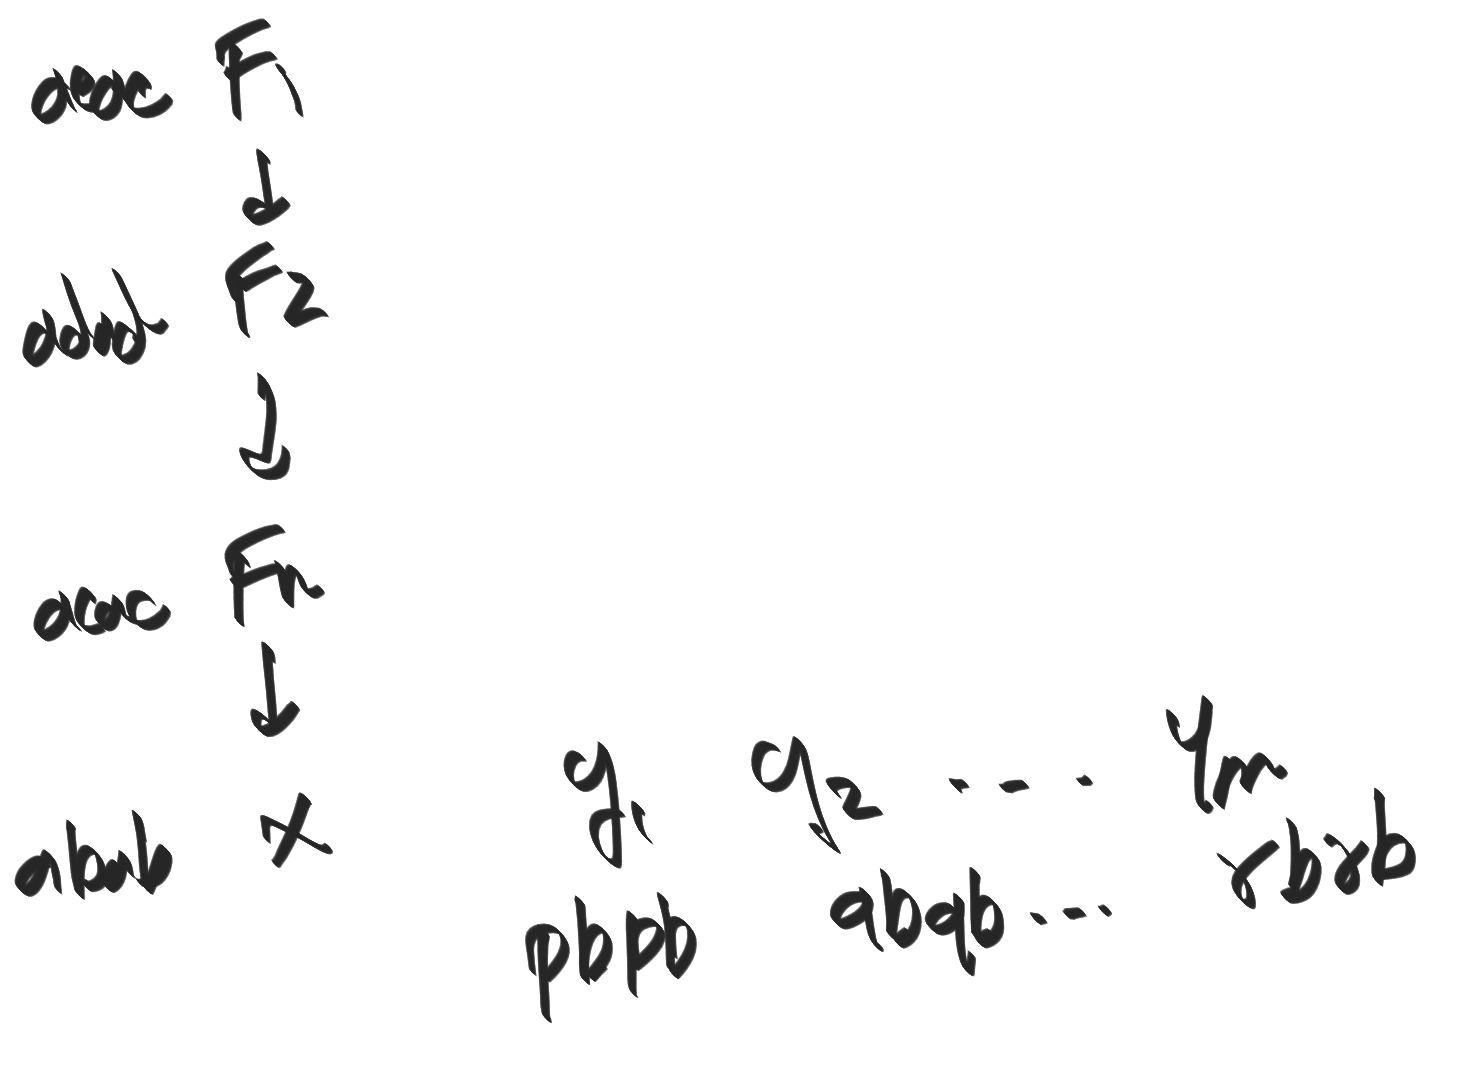
\includegraphics[width=\textwidth]{./eg-2-1.png}
\end{frame}

\begin{frame}[fragile]{Speedup over prior art: Merging}
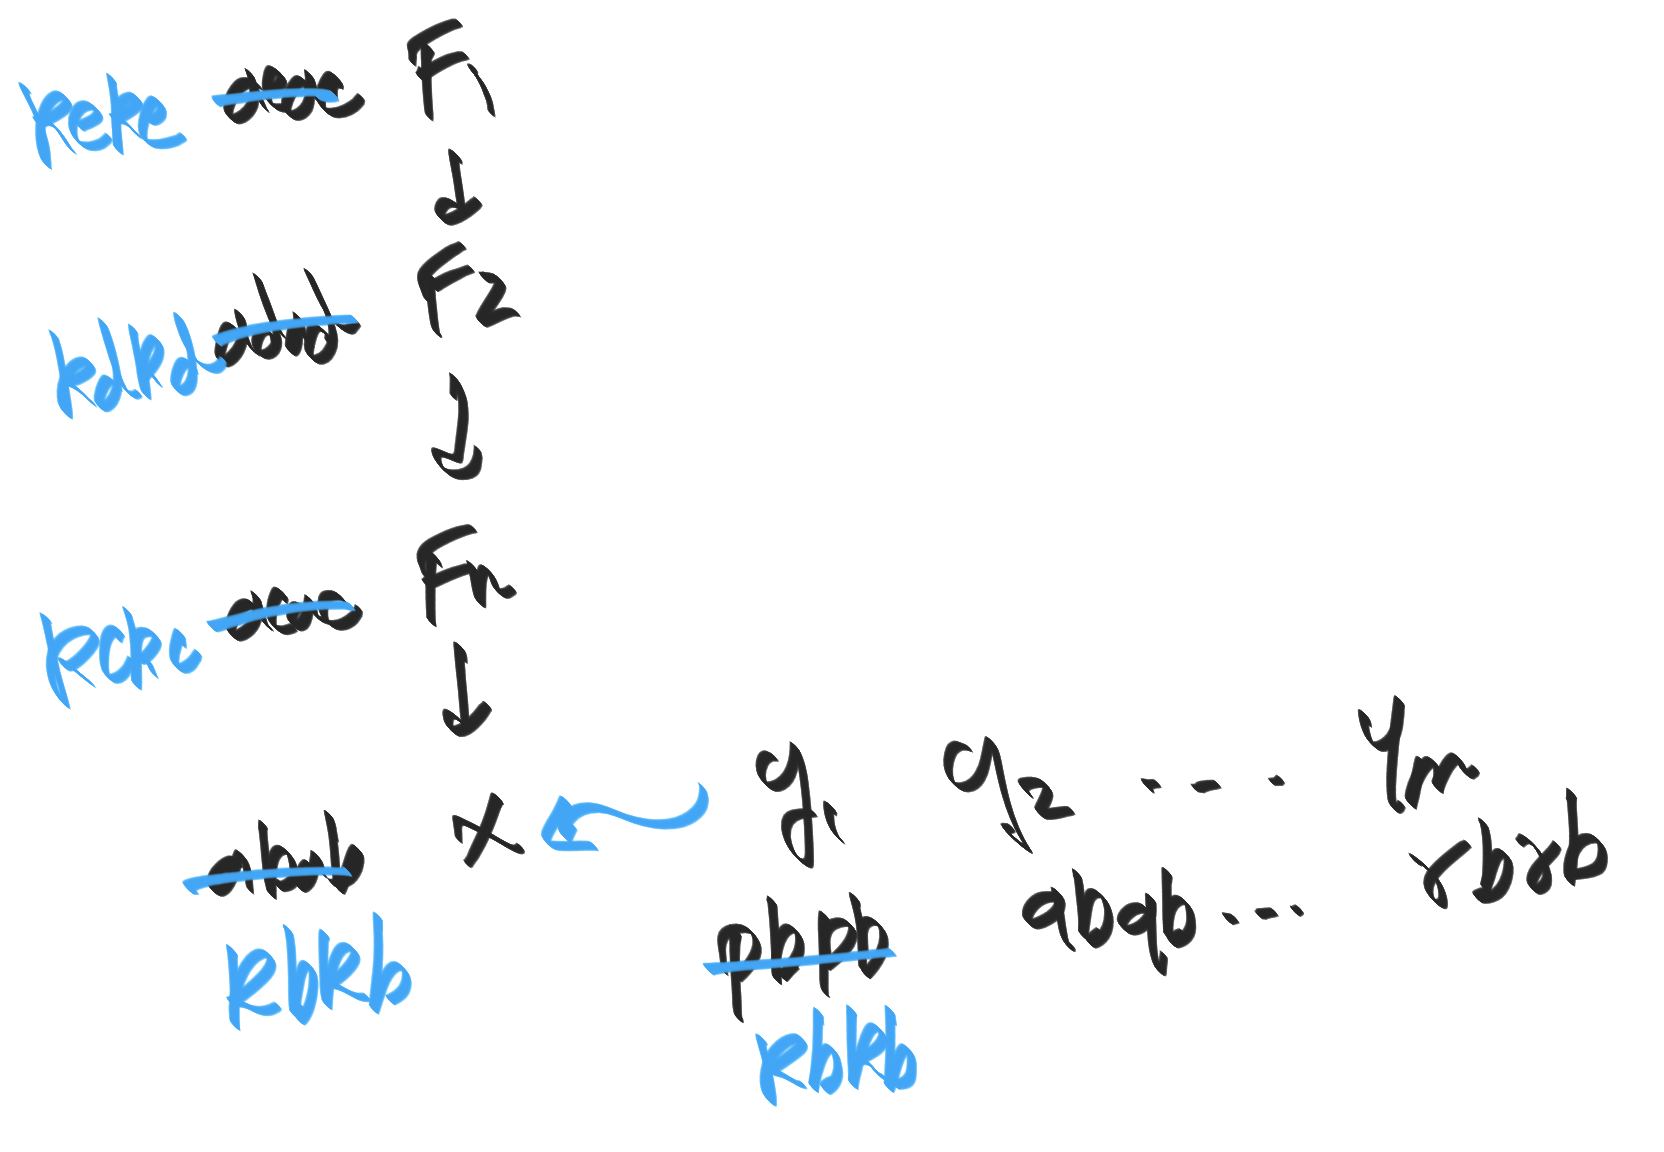
\includegraphics[width=\textwidth]{./eg-2-2.png}
\end{frame}

\begin{frame}[fragile]{Speedup over prior art: Merging}
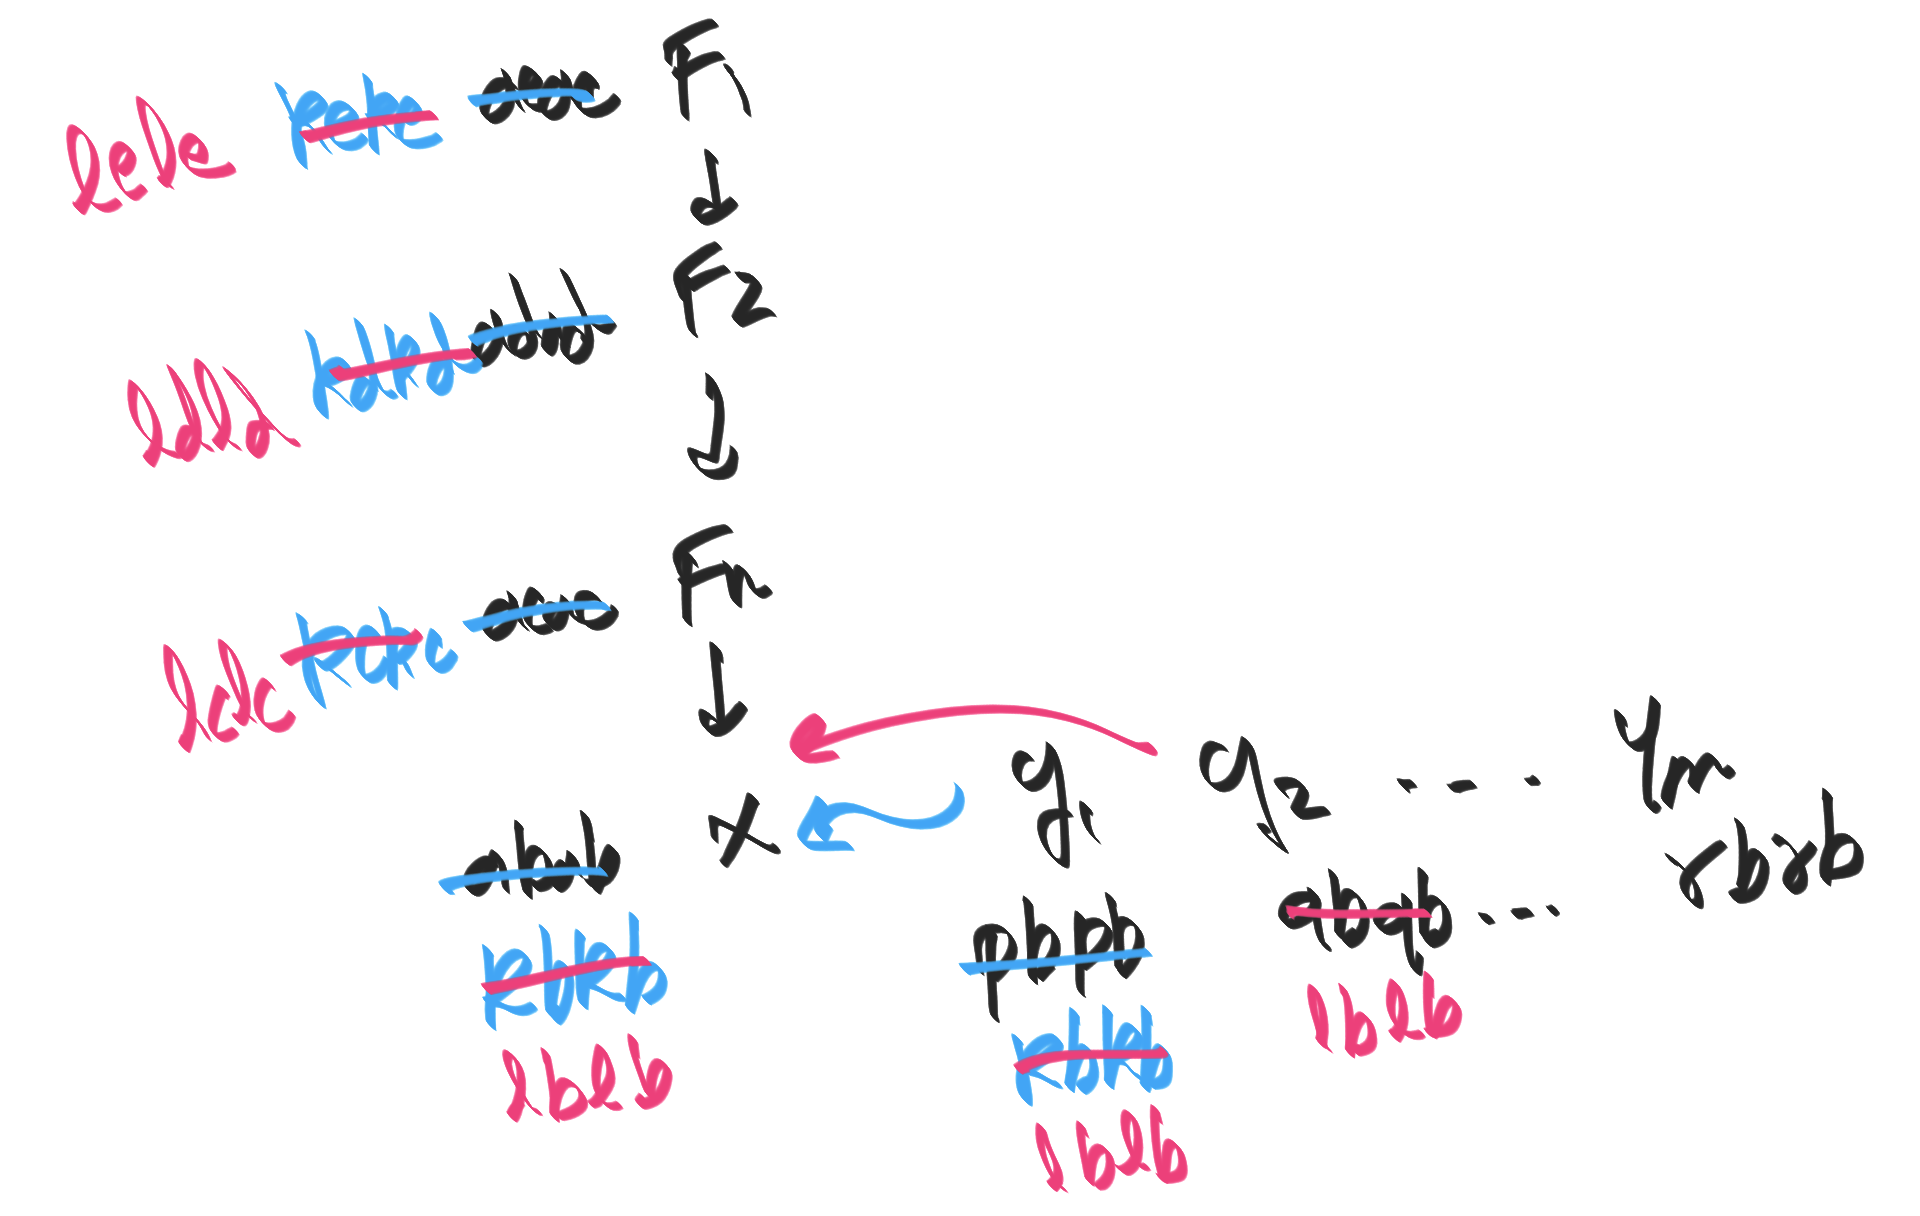
\includegraphics[width=\textwidth]{./eg-2-3.png}
\end{frame}

\begin{frame}[fragile]{Speedup over prior art: Merging}
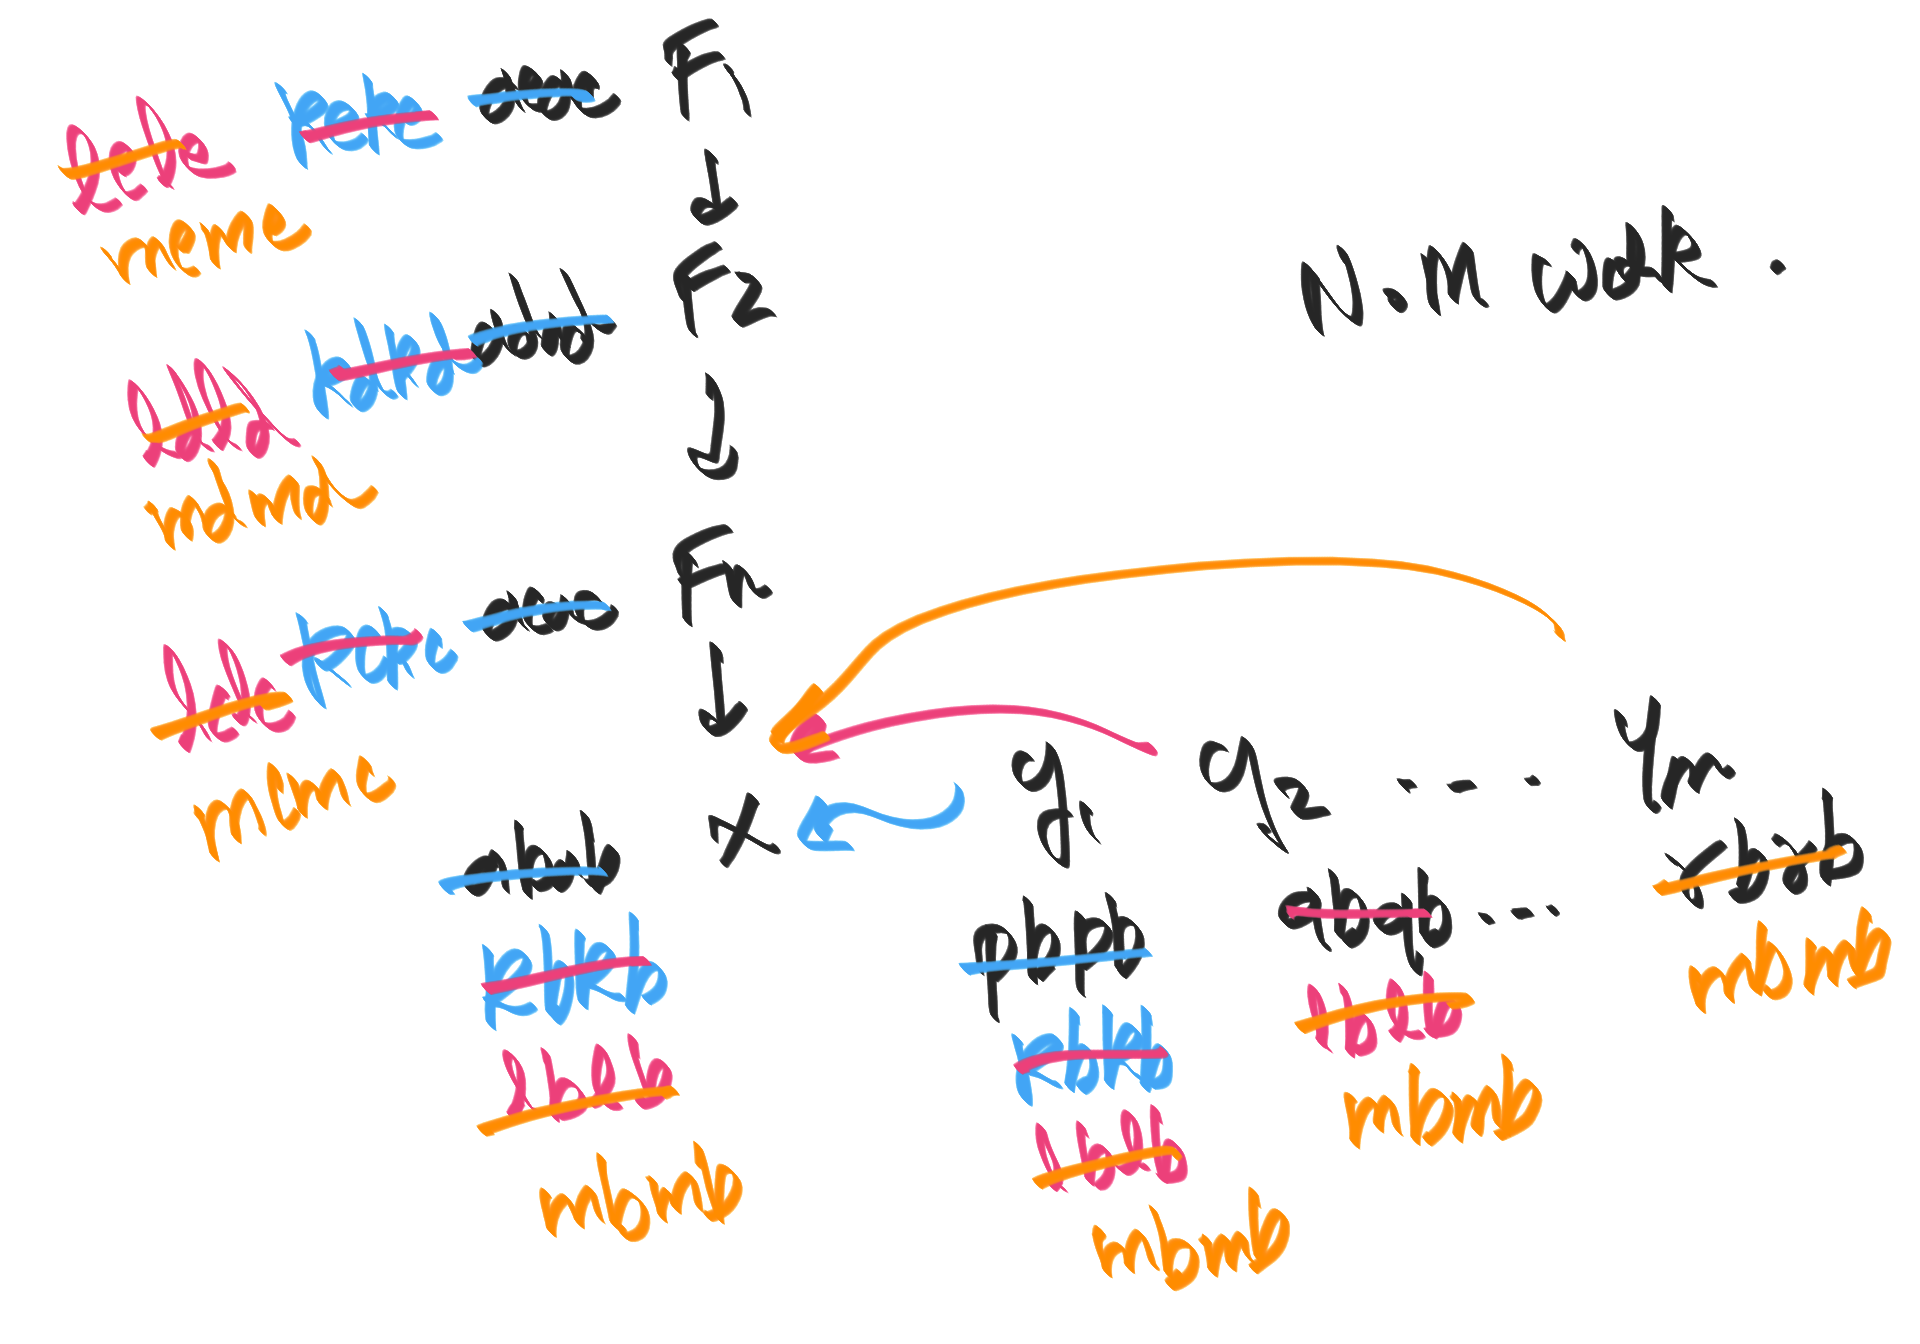
\includegraphics[width=\textwidth]{./eg-2-4.png}
\end{frame}


\begin{frame}[fragile]{Speedup over prior art: Merging}
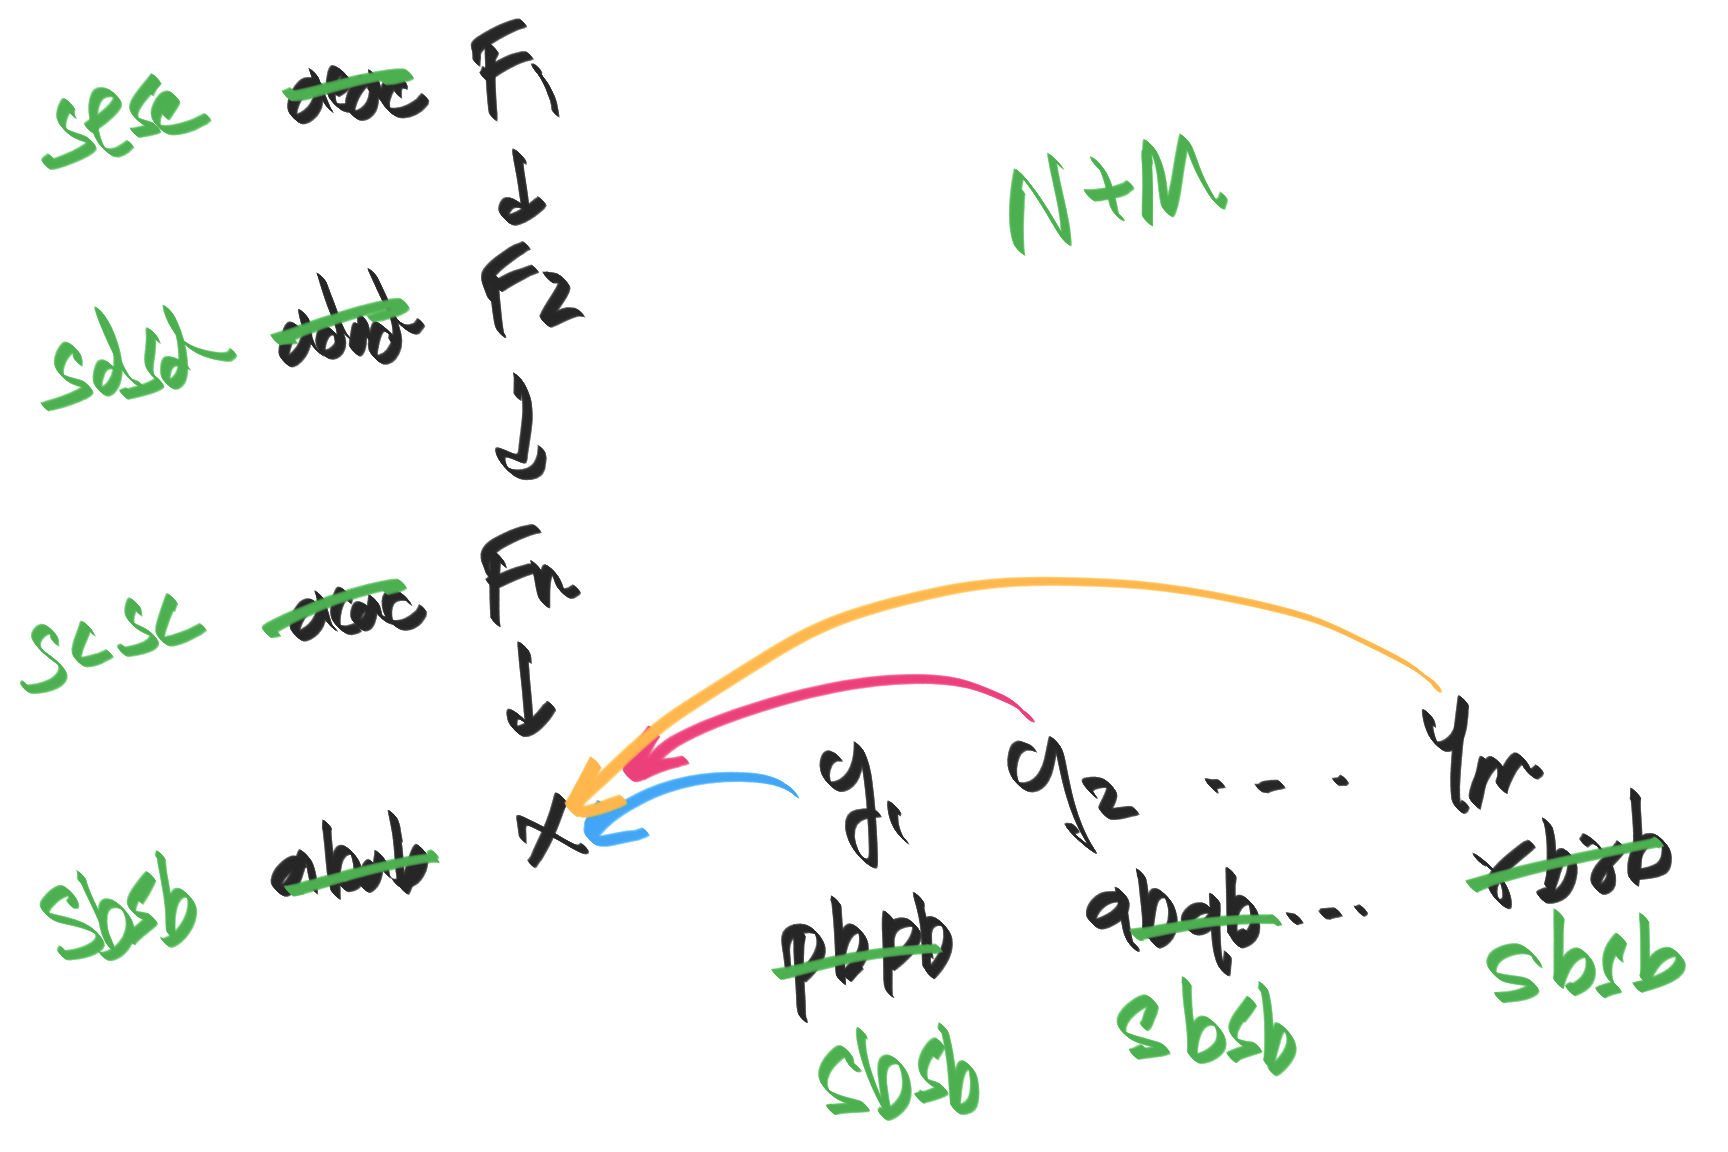
\includegraphics[width=\textwidth]{./eg-2-5.png}
\end{frame}



\begin{frame}[fragile]{Speedup over prior art: Merging}
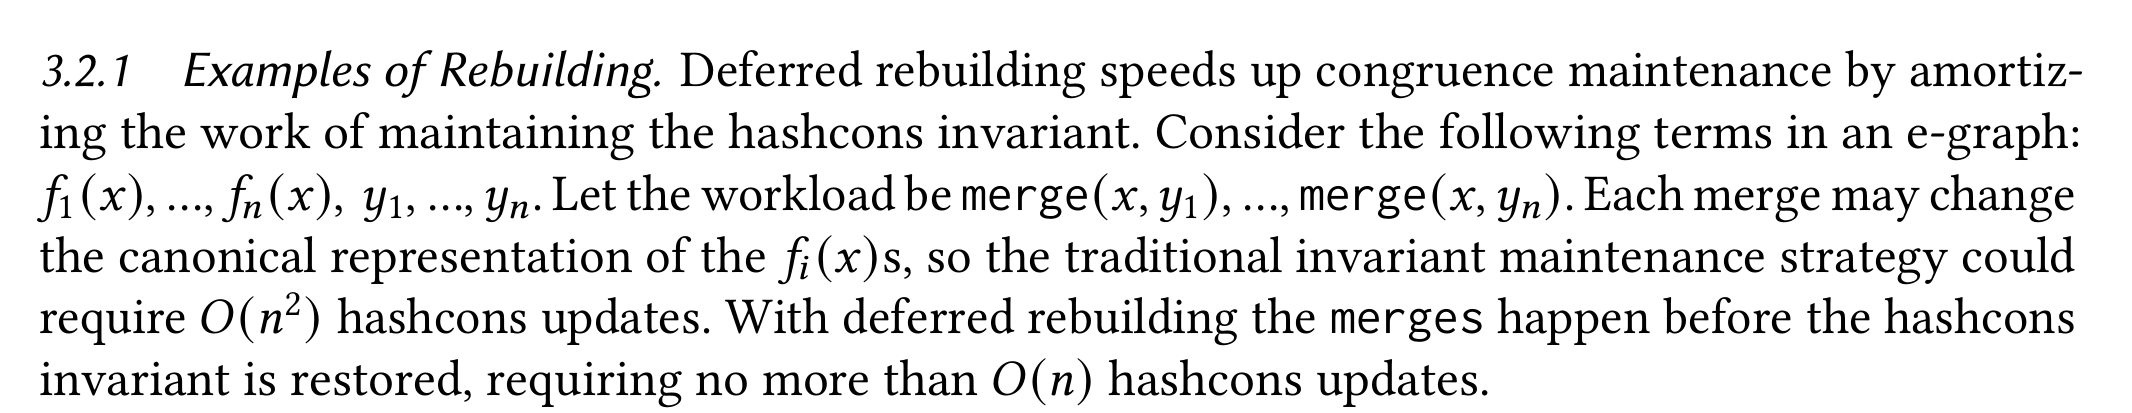
\includegraphics[width=\textwidth]{./eg-2-paper-snippet.png}
\end{frame}

\begin{frame}[fragile]{Analysis, formally}
\begin{itemize}
\item Abstract interpretation of equivalence classes.
\item For each node, provide function $\alpha: \node \rightarrow L$ (Abstraction function)
\item $(L, \cap)$ is a join-semilattice.
\item \egg provides for each equivalence class $\class \mapsto \bigcap_{\node \in \class} \alpha(\node) \in L$
\end{itemize}
\end{frame}


\begin{frame}[fragile]{Lambda calculus in \egg: Language}
\begin{minted}{rust}
define_language! {
  enum Lambda {
      Bool(bool),
      Num(i32),

      "var" = Var(Id),

      "+" = Add([Id; 2]),
      "=" = Eq([Id; 2]),

      "app" = App([Id; 2]),
      "lam" = Lambda([Id; 2]),
      "let" = Let([Id; 3]),
      "fix" = Fix([Id; 2]),

      "if" = If([Id; 3]),

      Symbol(egg::Symbol),
  }
}
\end{minted}

\end{frame}

\begin{frame}[fragile]{Lambda calculus in \egg: Analysis}
\begin{minted}{rust}
struct Data { free: HashSet<Id>, constant: Option<Lambda>, }
\end{minted}
\pause
\begin{minted}{rust}
impl Analysis<Lambda> for LambdaAnalysis {
    type Data = Data;
\end{minted}
\pause
\begin{minted}{rust}
    fn make(egraph: &EGraph, enode: &Lambda) -> Data {
        let f = |i: &Id| egraph[*i].data.free.iter().cloned();
        let mut free = HashSet::default();
\end{minted}
\pause
\begin{minted}{rust}
        match enode {
            Lambda::Var(v) => { // var
                free.insert(*v);
            }
\end{minted}
\pause
\begin{minted}{rust}
            Lambda::Let([v, a, b]) => { // let v = a in b(v)
                free.extend(f(b));
                free.remove(v);
                free.extend(f(a));
            }
\end{minted}
\pause
\begin{minted}{rust}
            // \v. a(v)
            Lambda::Lambda([v, a]) | Lambda::Fix([v, a]) => {
                free.extend(f(a));
                free.remove(v);
            }
            _ => enode.for_each(|c| free.extend(&egraph[c].data.free)),
        }
\end{minted}
\pause
\begin{minted}{rust}
        let constant = eval(egraph, enode);
        Data { constant, free }
    }
\end{minted}
\end{frame}


\begin{frame}[fragile]{Lambda calculus in \egg: Dynamic rewrites}

\begin{minted}{hs}
-- v2=x is not free in (\x. x + 1)
x_bound = let v1 = (\x. x*2) in (\x.   x+1)
x_bound = let v1 = e         in (\v2.  body)
\end{minted}
\pause
How to push \texttt{let} into \texttt{lambda}?
\pause
\begin{minted}{hs}
x_bound' = \x.  let v1 = (\x. x*2) in x + 1
x_bound' = \v2. let v1 = e         in body
\end{minted}
\pause
\begin{minted}{hs}
-- v2=x is free in e=x*2
x :: Int; x = 42
x_free = let v1 = x*2 in (\x.   x+1)
x_free = let v1 = e   in (\v2.  body)
\end{minted}
\pause
\begin{minted}{hs}
-- v2=x is free in e=x*2
x :: Int; x = 42
x_free'_wrong = \x. let v1 = x*2 in x + 1
\end{minted}
How to push \texttt{let} into \texttt{lambda}?
\pause
\begin{minted}{hs}
x :: Int; x = 42
x_free' = \fresh. let v1 = e   in (let v2 = fresh in body  )
x_free' = \fresh. let v1 = x*2 in (let x  = fresh in (x + 1))
\end{minted}
\pause
\end{frame}

\begin{frame}[fragile]{Lambda calculus in \egg: Dynamic rewrites}
\begin{minted}{hs}
x_free = let v1 = e   in (\v2.  body)
x_free' = \fresh. let v1 = e   in (let v2 = fresh in body  )
\end{minted}

\begin{minted}{rust}
rw!("let-lam-diff";
"(let ?v1 ?e (lam ?v2 ?body))" => // let v1 = e in \v2 . body
{ CaptureAvoid { // use an Applier called CaptureAvoid
    fresh: var("?fresh"), v2: var("?v2"), e: var("?e"),
    // \v2. let v1 = e in body
    if_not_free: "(lam ?v2 (let ?v1 ?e ?body))".parse().unwrap(),
    // \fresh. let v1 = e in let v2 = fresh in body 
    if_free: "(lam ?fresh (let ?v1 ?e (let ?v2 (var ?fresh) ?body)))"
      .parse().unwrap(),
}}
if is_not_same_var(var("?v1"), var("?v2"))),
\end{minted}
\end{frame}

\begin{frame}[fragile]{Lambda calculus in  \egg: Dynamic rewrites}
\begin{minted}{rust}
struct Data { free: HashSet<Id>, constant: Option<Lambda>, }
impl Analysis<Lambda> for LambdaAnalysis {
    type Data = Data;
    ...
\end{minted}
\pause
\begin{minted}{rust}
{ CaptureAvoid {  // rewrite pattern
    fresh: var("?fresh"), v2: var("?v2"), e: var("?e"),
    if_not_free: "(lam ?v2 (let ?v1 ?e ?body))".parse().unwrap(),
    if_free: "(lam ?fresh (let ?v1 ?e (let ?v2 (var ?fresh) ?body)))"
        .parse().unwrap(),
}}
\end{minted}
\pause
\begin{minted}{rust}
struct CaptureAvoid {
    fresh: Var, v2: Var, e: Var,
    if_not_free: Pattern<Lambda>,
    if_free: Pattern<Lambda>,
}
\end{minted}
\pause
\begin{minted}{rust}
impl Applier<Lambda, LambdaAnalysis> for CaptureAvoid {
    fn apply_one(&self, egraph: &mut EGraph, eclass: Id, subst: &Subst) ...

        let e = subst[self.e];
        let v2 = subst[self.v2];
        let v2_free_in_e = egraph[e].data.free.contains(&v2);
\end{minted}
\pause
\begin{minted}{rust}
        if v2_free_in_e { ...  } else { ...  }
\end{minted}
\end{frame}


\begin{frame}{Conclusion}
\begin{itemize}
\item Use equalities to find equivalent programs.
\item Extract out the best program using a local analysis.
\item Analysis + Rewrites in a single unified framework.
\end{itemize}
\end{frame}

% \begin{frame}{Lambda calculus in \egg: constant folding}
% \begin{minted}{rust}
% fn eval(egraph: &EGraph, enode: &Lambda) -> Option<Lambda> {
%     let x = |i: &Id| egraph[*i].data.constant.clone();
%     match enode {
%         Lambda::Num(_) | Lambda::Bool(_) => Some(enode.clone()),
%         Lambda::Add([a, b]) => Some(Lambda::Num(x(a)?.num()? + x(b)?.num()?)),
%         Lambda::Eq([a, b]) => Some(Lambda::Bool(x(a)? == x(b)?)),
%         _ => None,
%     }
% }
% \end{minted}
% \end{frame}

\end{document}
